\documentclass{csnotes}

% ==============================================================================
% DOCUMENT SPECIFIC CUSTOMIZATIONS
% ==============================================================================

% --------------------------- START CUSTOMIZATIONS -----------------------------

% You can add any custom packages or commands specific to this document here
\newcommand{\SCal}{\mathcal{S}}
\setabstracttitle{Scopo del documento}

% ---------------------------- END CUSTOMIZATIONS ------------------------------



% ==============================================================================
% DOCUMENT INFORMATION
% ==============================================================================
\title{Encoding \& Encryption}
\author{Riccardo Elena, Fabrizio Apuzzo}
\date{\today}

% Additional information for the title page
\university{Università degli Studi Federico II di Napoli}
\department{Dipartimento d'Ingegneria Elettrica e Tecnologie dell'Informazione}
\course{Corso di Laurea Magistrale in Computer Science}
\subject{Encoding \& Encryption}
\academicyear{Anno Accademico 2024/2025}

% ==============================================================================
% BIBLIOGRAPHY
% ==============================================================================
% Specify the .bib file with your bibliographic references
% Uncomment the following line when you have created the bibliography.bib file
% \addbibresource{bibliography.bib}

% ==============================================================================
% INIZIO DOCUMENTO
% ==============================================================================

\begin{document}


\maketitlepage{}


\tableofcontents
\newpage

\begin{abstract}
  Appunti del corso di Encoding \& Encryption tenuto dal Prof. Alessandro De Luca.
\end{abstract}
\chapter{Prerequisiti di Algebra}

Prima di iniziare a trattare gli argomenti principali del corso,
è necessario ripassare alcuni concetti di algebra alla base della teoria dei codici introducendone alcuni nuovi.

In particolare questo capitolo si concentra sulle strutture algebriche di semigruppi e monoidi.

Prima di addentrarci nelle definizioni delle suddette strutture algebriche, è necessario introdurre alcune nozioni preliminari, che verranno conservate per tutto il corso di questi appunti.

\section{Nozioni Preliminari}

Le lettere maiuscole \(A, B, X, Y \ldots\) indicheranno generalmente insiemi, che siano finiti o infiniti.
Per quanto riguarda gli insiemi numerici tradizionali, useremo:
\begin{itemize}
  \item \(\N = \set{0,1,2,\ldots}\) per i numeri naturali (incluso lo zero);
  \item \(\N_+ = \set{1,2,3,\ldots}\) per i numeri naturali positivi (escluso lo zero);
  \item \(\Z\) per i numeri interi;
  \item \(\Q\) per i numeri razionali;
  \item \(\R\) per i numeri reali.
\end{itemize}
Con eventuali notazioni aggiuntive a pedice per indicare sottoinsiemi particolari (ad esempio \(\R_{\geq 0}\) per i numeri reali non negativi).

Per ogni insieme \(X\), \(\mathcal{P}(X)\) denota l'insieme delle parti di \(X\), ovvero l'insieme di tutti i sottoinsiemi di \(X\) e \(\#X\) la sua cardinalità.
Gli elementi di tali insiemi saranno indicati con le lettere minuscole corrispondenti \(a,b,x,y \ldots\), in particolare con la lettera \(n\) a indicare un generico elemento naturale se non specificato diversamente.

\section{Semigruppi e Monoidi}
\begin{definition}[Semigruppo]
  Un \keyword{semigruppo} è una coppia \((S, \cdot)\) dove \(S\) è un insieme non vuoto e \(\cdot : S \times S \to S\) è un'operazione binaria associativa, ovvero:
  \[\forall a,b,c \in S, (a \cdot b) \cdot c = a \cdot (b \cdot c).\]
\end{definition}

Questa struttura algebrica è molto generica, imponendo solo l'associatività dell'operazione binaria.
Un esempio di semigruppo è dato da \((\N',+)\) dove l'operazione binaria è la somma tra numeri naturali positivi ordinaria.

\begin{definition}[Monoide]
  Un \keyword{monoide} \((M,\cdot,1_M)\) è un semigruppo \((M, \cdot)\) dotato di elemento neutro \(1_M\) per l'operazione binaria\footnote{Denotato semplicemente \(1\) in caso di non ambiguità del monoide di riferimento}, ovvero:
  \[\forall a \in M, a \cdot 1_M = 1_M \cdot a = a.\]
\end{definition}

\begin{example}
  \begin{itemize}
    \item \((\N, +)\) è un monoide con elemento neutro \(0\).
    \item \((\N, \cdot)\) è un monoide con elemento neutro \(1\).
    \item Dato \(T\) insieme, sia \((\mathcal{P}(T), \cup, \emptyset)\) che \((\mathcal{P}(T), \cap, T)\) sono monoidi.
  \end{itemize}
  Gli esempi precedenti sono tutti monoidi commutativi (o abeliani), ovvero tali che:
  \[\forall a,b \in M, a \cdot b = b \cdot a.\]
  Un esempio di monoide non abeliano è, dato un insieme \(T\), il monoide delle funzioni totali da \(T\) in sé stesso \((T^{T}, \circ, id_T)\) dove l'operazione binaria è la composizione di funzioni e l'elemento neutro è la funzione identità su \(T\).
\end{example}

\subsection{Proprietà di monoidi e semigruppi}

Analizziamo ora alcune notazioni e proprietà di monoidi e semigruppi.

\begin{note}\label{note:power_notation}
  Dato \((M,\cdot,1_M)\) monoide, si ha che, \(\forall m \in M\), \(m^0 = 1_M\) e \(m^{n+1} = m \cdot m^n, \quad \forall n \geq 0\).
\end{note}

\begin{definition}[Morfismi di semigruppi e monoidi]
  Siano \((S,\cdot)\) e \((T,*)\) semigruppi.
  Una funzione \(f: S \to T\) è un \keyword{morfismo di semigruppi} se:
  \[\forall a,b \in S, f(a \cdot b) = f(a) * f(b).\]
  Se \(S\) e \(T\) sono monoidi, \(f\) è un \keyword{morfismo di monoidi} se è un morfismo di semigruppi e:
  \[f(1_S) = 1_T.\]
  Se \(f\) è iniettiva, si dice che è un \keyword{monomorfismo}, se è suriettiva si dice che è un \keyword{epimorfismo}, se è biunivoca si dice che è un \keyword{isomorfismo}.
  In quest'ultimo caso, i due semigruppi (o monoidi) si dicono isomorfi.
\end{definition}
\begin{example}
  Consideriamo i monoidi \((\N, +, 0)\) e \((\N, \cdot, 1)\).
  La funzione 
  \[f: \N \to \N\]
  \[f:n \mapsto f(n) = 2^n\]
  è un monomorfismo tra i due monoidi.
  Infatti,
  \[f(n+m) = 2^{n+m} = 2^n \cdot 2^m = f(n) \cdot f(m)\]
  \[ f(0) = 2^0 = 1\]
  Tuttavia, \(f\) non è un epimorfismo, poiché non è suriettiva (ad esempio, non esiste \(n \in \N\) tale che \(f(n) = 3\)).
\end{example}

\begin{definition}[Sottosemigruppo e Sottomonoide]
  Sia \((S,\cdot_S)\) un semigruppo.
  \(T \subseteq S\) è un \keyword{sottosemigruppo} di \(S\) (\(T \leq S\)), se \(T\) è chiusa rispetto all'operazione binaria di \(S\), ovvero:
  \[\forall a,b \in T, a \cdot_S b \in T\]
  Dato \((M,\cdot_M,1_M)\) è un monoide, \(N \subseteq M\) è un \keyword{sottomonoide} di \(M\) (\(N \leq M\)) se:
  \begin{itemize}
    \item \(N\) è un sottosemigruppo di \(M\);
    \item \(1_M \in N\).
  \end{itemize}
\end{definition}

Dato un qualsiasi semigruppo \((S,\cdot)\), è possibile costruire un semigruppo sul suo insieme delle parti \(\mathcal{P}(S)\) indotto dall'operazione binaria di \(S\).
\begin{definition}[Semigruppo delle parti]
  Sia \((S,\cdot)\) un semigruppo.
  Definiamo l'operazione binaria \(\circ\) su \(\mathcal{P}(S)\) come:
  \[\forall X,Y \in \mathcal{P}(S), X \circ Y = \set{x \cdot y}[ x \in X, y \in Y].\]
\end{definition}
Tale costruzione è estendibile anche a un qualsiasi monoide \((M,\cdot,1_M)\), usando come elemento neutro l'insieme \(\set{1_M}\).

Questo semigruppo (o monoide) delle parti è particolarmente rilevante, poiché, grazie alle notazioni introdotte nella Nota~\ref{note:power_notation}, è possibile definire le potenze di un qualsiasi sottoinsieme \(Y \subseteq S\).

Tale notazione permette di formulare in modo più compatto la chiusura di un sottoinsieme \(Y\) di un semigruppo.
  \[(\forall a,b \in T, a \cdot_S b \in T)\iff (Y^2 \subseteq Y).\]
\begin{proof}[Idea di dimostrazione]\label{proof:alt_notation_closure}
  Da definizione infatti, \(Y^2 = \set{y_1 \cdot y_2}[y_1,y_2 \in Y]\). Se \(Y^2 \subseteq Y\), allora anche \(Y^3 = Y^2 \cdot Y \subseteq Y\), poiché
  \[\forall y \in Y^3, \exists y_1 \in Y, y_2 \in Y^2\st y = y_1 \cdot y_2\]
  Iterando il ragionamento è possibile mostrare che \(Y\) contiene tutte le potenze di sé stesso, ed è dunque chiuso.
\end{proof}

\begin{definition}[Sottostruttura generata]
  Sia \((S,\cdot)\) un semigruppo e \(Y \subseteq S\).
  Definiamo il \keyword{sottosemigruppo} di \(S\) generato da \(Y\) come:
  \[Y^+ = Y \cup Y^2 \cup Y^3 \cup \cdots = \bigcup_{n=1}^{\infty} Y^n\]
  l'insieme di tutte le possibili combinazioni finite di elementi di \(Y\) tramite l'operazione binaria di \(S\).

  Dato \((M,\cdot_M,1_M)\) monoide, è possibile aggiungere la potenza zero, definendo il \keyword{sottomonoide} di \(M\) generato da \(Y\) come:
  \[Y^* = \set{1_S} \cup Y^+ = \bigcup_{n=0}^{\infty} Y^n.\]
\end{definition}

Tali sottostrutture sono le più piccole possibili che contengono \(Y\).\\
Un monoide notevole per il corso è il cosiddetto \emph{monoide delle parole}.
Dato un insieme finito \(A\), detto \emph{alfabeto}, l'insieme di tutte le possibili sequenze finite (dette stringhe o parole) di elementi di \(A\) forma un monoide rispetto all'operazione di concatenazione di stringhe. 
Tale monoide contiene \(A\) e ha come elemento neutro la stringa vuota, indicata con \(\varepsilon\).
Denotiamo tale monoide con \(A^*\), e l'insieme delle stringhe non vuote con \(A^+ = A^* \setminus \set\varepsilon\).

\begin{example}
  Sia \(A = \set{0,1}\) un alfabeto binario.
  Allora \(A^* = \set{\varepsilon, 0, 1, 00, 01, 10, 11, 000, \ldots}\) è il monoide delle parole binarie.
  Si noti che \(A^*\) è infinito anche se \(A\) è finito.
\end{example}

\begin{definition}[Base di un semigruppo (monoide)]
  Sia \(S\) un semigruppo (monoide).
  Una \keyword{base} di \(S\) è un sottoinsieme \(X \subseteq S\) che gode di \emph{univoca fattorizzazione}, ovvero che dati \(\forall x_1,x_2,\ldots,x_n,x_1',x_2',\ldots,x_m' \in X\) si ha che:
  \[x_1 x_2 \ldots x_n = x_1' x_2' \ldots x_m' \implies n=m \land x_1 = x_1' \land x_2 = x_2' \land \ldots \land x_n = x_n'\]
\end{definition}
In altre parole, ogni elemento di \(X^{+}\) si fattorizza in un unico modo come prodotto di elementi di \(X\).

\begin{example}
  Esempi di basi sono:
  \begin{itemize}
    \item \(A\) è una base di \(A^*\) per ogni alfabeto \(A\).
    \item \(\set{1}\) è una base di \((\N, +, 0)\).
  \end{itemize}
  Contrariamente a quello che si potrebbe pensare, l'insieme dei numeri primi \textbf{non} è una base di \((\N, \cdot, 1)\), poiché \(6 = 2 \cdot 3 = 3 \cdot 2\) ammette due fattorizzazioni distinte.
\end{example}

\begin{note}\label{note:no_neutral_in_base}
  Per definizione di base, nessuna base di un monoide può contenere l'elemento neutro.
  Infatti, se \(1_M \in X\), \(\forall x \in X\) si ha che \(1_M \cdot x = x\), quindi ogni elemento di \(X^{+}\) si fattorizza in un modo non univoco.
\end{note}

\begin{definition}[Semigruppi e monoidi liberi]
  Data \(X \subseteq S\) base di un semigruppo \(S\), si dice che \(S\) è \keyword{libero} se \(S = X^{+}\).
  Analogamente, dato \(X \subseteq M\) base di un monoide \(M\), si dice che \(M\) è \keyword{libero} se \(M = X^{*}\).
\end{definition}
Una modo meno formale ma più intuitivo di definire un semigruppo (monoide) libero è quella di considerarlo il semigruppo (monoide) con la minor quantità di vincoli possibile, ovvero solo quelli imposti dalla definizione di semigruppo (monoide).
La struttura è \emph{libera} poiché non ha vincoli aggiuntivi che la limitano, essendo dunque la più generale possibile dato l'insieme sottostante.
Tale proprietà di generalità verrà formalizzata più avanti tramite una proprietà universale.

\todo{Chiedere a De Luca se \((\N,+)\) è libero di base \(\set{1}\), se no perché? Neanche isomorfo a \(\set{1}^*\)? Non è sufficiente?}
Un esempio di monoide libero è il monoide delle parole \(A^*\) per ogni alfabeto \(A\), che è libero di base \(A\).

\begin{proposition}[Unicità della base in un semigruppo (monoide) libero]
  Sia \(S\) un semigruppo libero, allora l'unica base di \(S\) è \(S \setminus S^2\), ovvero l'insieme degli elementi di \(S\) che non sono esprimibili come prodotto di altri elementi di \(S\).
  Analogamente, sia \(M\) un monoide libero, allora l'unica base di \(M\) è \((M\setminus \{1_M\}) \setminus {(M\setminus \{1_M\})}^2\).
\end{proposition}
\begin{proof}[Idea di dimostrazione]
  Analogo a~\ref{proof:alt_notation_closure}
\end{proof}

\begin{theorem}[Proprietà universale dei monoidi (semigruppi) liberi]
  Sia \(M\) un monoide con \(X \subseteq M\). Allora \(M\) è libero di base \(X\) se e solo se, per ogni monoide \(M'\) e ogni applicazione \(f: X \to M'\), esiste un unico morfismo di monoidi \(\bar{f}: M \to M'\) tale che \(\hat{f}_{|_X} = f\), ovvero tale che il seguente diagramma commuta:
  \begin{center}
      \begin{tikzcd}[column sep=huge, row sep=huge, cells={nodes={scale=1.2, transform shape}}]
        X \arrow[r, "f"] \arrow[d, hook,"i"] & M' \\ %chktex 18 
        M \arrow[ru, dashed, "\exists!\bar{f}"'] & %chktex 18
      \end{tikzcd}
  \end{center}
  Vale a dire che \(\bar{f} \circ i = f\), dove \(i: X \hookrightarrow M\) è l'inclusione di \(X\) in \(M\).\footnote{È possibile vedere \(i\) anche come la riduzione dell'identità di \(M\) a \(X\), ovvero \(i = id_{M|_X}\).}
  Tale formulazione ha carattere algebrico-universale e quindi può essere estesa anche ai semigruppi, oltre che a qualsiasi famiglia di algebre dello stesso tipo, quali per esempio i gruppi.
\end{theorem}

È importante notare che la proprietà universale, dato un monoide \(M\) e una sua base \(X\) vale \emph{per ogni monoide \(M'\)}, e quindi in particolare anche per \(M' = M\).
Da questa particolare circostanza è facile ricavare che \(id_M: M \to M\) è l'unico morfismo da \(M\) a \(M\) che estende \(id_X\).

\begin{corollary}
  Sia \(M\) monoide libero di base \(X\) e \(M'\) monoide libero di base \(X'\).
  Se \(\#X = \#X'\), allora \(M\) e \(M'\) sono isomorfi.
\end{corollary}

\begin{proof}
  Per dimostrare tale corollario sarà sufficiente mostrare che è possibile costruire un morfismo biettivo (isomorfismo) tra \(M\) e \(M'\)
  Essendo le basi equipotenti, esiste una biiezione \(g: X \to X'\).
  Consideriamo l'applicazione \(f = i' \circ g : X \to M'\), dove \(i': X' \hookrightarrow M'\), ovvero l'inclusione di \(X'\) in \(M'\).
  Per la proprietà universale, esiste un unico morfismo di monoidi \(\bar{f}: M \to M'\) tale che \(\bar{f}_{|_X} = f\).
  Analogamente, sia \(f'= i \circ g^{-1} : X' \to M\) e sia \(\bar{f'}: M' \to M\) l'unico morfismo di monoidi tale che \(\bar{f'}_{|_{X'}} = f'\).
  Si ha che \(\bar{f'} \circ \bar{f}: M \to M\) è un morfismo di monoidi che estende \(id_X\), ovvero:
  \[\forall x \in X, \bar{f'} (\bar{f}(x)) = \bar{f'}(g(x))= g^{-1}(g(x))= x\]
  Come detto precedentemente però \(id_M\) è l'unico morfismo di monoidi da \(M\) in sé stesso che estende \(id_X\), dunque necessariamente si ha che \(\bar{f'} \circ \bar{f} = id_M\)
  Dalla definizione di biettività abbiamo che \(\bar{f} = \bar{f'}^{-1} \), ovvero che \(\bar{f}\) è un isomorfismo tra \(M\) e \(M'\). 
\end{proof}
Questo corollario mostra che, a meno di isomorfismi, il monoide libero \(A^*\) è l'unico monoide libero con base di cardinalità \(\#A\).

Dato un monoide libero \(M\) è possibile definire un morfismo di lunghezza delle parole.
\begin{definition}[Morfismo di lunghezza]
  Sia \(M\) un monoide libero di base \(X\).
  Il \keyword{morfismo di lunghezza} è \(|\;|: M \to(\N,+,0)\) tale che \[\forall x \in X, |x| = 1\]
\end{definition}

\begin{note}
  È importate notare che il morfismo di lunghezza è ben definito per ogni valore di \(M\), poiché ogni elemento di \(M\) si fattorizza in modo univoco come prodotto di elementi di \(X\).
  Non fosse stato così, non sarebbe possibile definire in modo univoco la lunghezza di un elemento di \(M\) a partire dagli elementi della sua base.
\end{note}

\begin{lemma}[Levi]\label{thm:levi}
  Sia \(M\) un monoide libero, \(m_1,m_2,m_3,m_4 \in M\) tali che \(m_1m_2=m_3m_4 \text{ e } |m_1| \geq |m_3|\).
  Allora \(\exists v \in M: m_1 = m_3v \land vm_2 = m_4\)
\end{lemma}

\begin{proof}
  Chiamiamo \(w\) la parola comune \(m_1m_2 = m_3m_4\).
  Possiamo rappresentare la sua fattorizzazione in \(m_1m_2\) come:
  \begin{figure}[H]
    \centering
    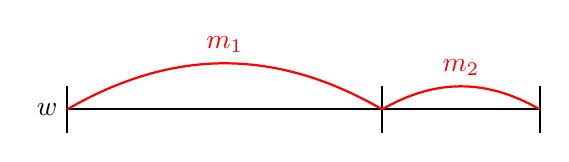
\begin{tikzpicture}
      \coordinate (A) at (0,0);
      \coordinate (B) at (6,0);
      \draw[thick] (A) -- (B);
      \foreach \x in {0,4,6}{
        \coordinate (P\x) at (\x,0);
        \draw[thick] (P\x) -- ++(0,-0.3);
        \draw[thick] (P\x) -- ++(0,0.3);
      }
      \node[left] at (A) {\(w\)};
      \draw[thick, red, bend left] (A) to node[midway, above, red] {\(m_1\)} (P4);
      \draw[thick, red,bend left] (P4) to node[midway, above, red] {\(m_2\)} (P6);
    \end{tikzpicture}
  \end{figure}
  e la fattorizzazione in \(m_3m_4\) come:
  \begin{figure}[H]
    \centering
    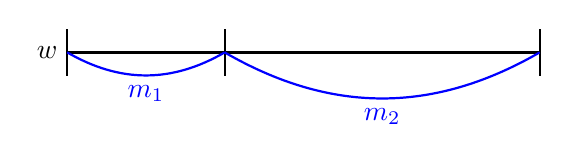
\begin{tikzpicture}
      \coordinate (A) at (0,0);
      \coordinate (B) at (6,0);
      \draw[thick] (A) -- (B);
      \foreach \x in {0,2,6}{
        \coordinate (P\x) at (\x,0);
        \draw[thick] (P\x) -- ++(0,-0.3);
        \draw[thick] (P\x) -- ++(0,0.3);
      }
      \node[left] at (A) {\(w\)};
      \draw[thick, blue,bend right] (A) to node[midway, below, blue] {\(m_1\)} (P2);
      \draw[thick, blue,bend right] (P2) to node[midway, below, blue] {\(m_2\)} (P6);
    \end{tikzpicture}
  \end{figure}
  Se \(\abs{m_1} = \abs{m_3}\), dall'ipotesi che \(M\) è libero segue che \(m_1 = m_3\) e \(m_2 = m_4\).
  Questo perché, non fossero uguali, si avrebbe una doppia fattorizzazione di \(w\), in contraddizione con la definizione di base.
  Il teorema in questo caso è verificato ponendo \(v = \varepsilon\).

  Nel caso \(\abs{m_1} > \abs{m_3}\) invece, il punto di divisione tra \(m_1\) e \(m_2\) si trova a destra del punto di divisione tra \(m_3\) e \(m_4\).
  Di conseguenza, è possibile sovrapporre le rappresentazioni precedenti come segue:
  \begin{figure}[H]
    \centering
    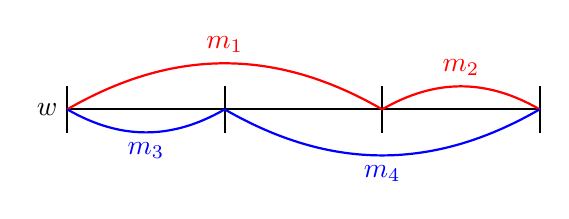
\begin{tikzpicture}
      \coordinate (A) at (0,0);
      \coordinate (B) at (6,0);
      \draw[thick] (A) -- (B);
      \foreach \x in {0,2,4,6}{
        \coordinate (P\x) at (\x,0);
        \draw[thick] (P\x) -- ++(0,-0.3);
        \draw[thick] (P\x) -- ++(0,0.3);
      }
      \node[left] at (A) {\(w\)};
      \draw[thick, red, bend left] (A) to node[midway, above, red] {\(m_1\)} (P4);
      \draw[thick, red,bend left] (P4) to node[midway, above, red] {\(m_2\)} (P6);
      \draw[thick, blue,bend right] (A) to node[midway, below, blue] {\(m_3\)} (P2);
      \draw[thick, blue,bend right] (P2) to node[midway, below, blue] {\(m_4\)} (P6);
    \end{tikzpicture}
  \end{figure}
  Chiamando \(v\) la parola compresa tra i due punti di divisione si ha che \(m_1 = m_3v\) e \(vm_2 = m_4\).
  Anche in questo caso, se una delle due uguaglianze non fosse verificata, si avrebbe una doppia fattorizzazione di \(w\), in contraddizione con la definizione di base.
  \begin{figure}
    \centering
    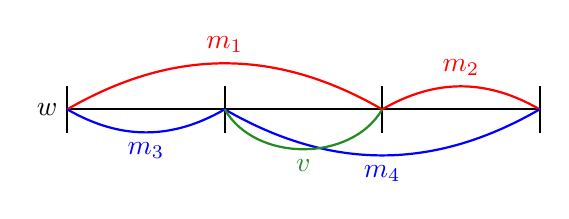
\begin{tikzpicture}
      \coordinate (A) at (0,0);
      \coordinate (B) at (6,0);
      \draw[thick] (A) -- (B);
      \foreach \x in {0,2,4,6}{
        \coordinate (P\x) at (\x,0);
        \draw[thick] (P\x) -- ++(0,-0.3);
        \draw[thick] (P\x) -- ++(0,0.3);
      }
      \node[left] at (A) {\(w\)};
      \draw[thick, red, bend left] (A) to node[midway, above, red] {\(m_1\)} (P4);
      \draw[thick, red,bend left] (P4) to node[midway, above, red] {\(m_2\)} (P6);
      \draw[thick, blue,bend right] (A) to node[midway, below, blue] {\(m_3\)} (P2);
      \draw[thick, blue,bend right] (P2) to node[midway, below, blue] {\(m_4\)} (P6);
      \draw[thick, ForestGreen, bend right=60] (P2) to node[midway, below, ForestGreen] {\(v\)} (P4);
    \end{tikzpicture}
  \end{figure}
  
  
\end{proof}

\begin{definition}[Insiemi quoziente]\label{def:quotien_set}
  Siano \(Y,Z \subseteq M\) monoide. Definiamo gli insieme quoziente destro e sinistro come:
  \begin{equation}
    \begin{aligned}
      Y^{-1}Z &= \set{m \in M}[ \exists y \in Y, ym \in Z] = \set{m \in M}[Y\set{m} \cap Z \neq \emptyset]\\
      ZY^{-1} &= \set{m \in M}[ \exists y \in Y, my \in Z] = \set{m \in M}[\set{m}Y \cap Z \neq \emptyset]
    \end{aligned}
  \end{equation}
\end{definition}

In altre parole possiamo vedere l'insieme quoziente sinistro (rispettivamente destro) come l'insieme delle parole di \(M\) che servono a completare a sinistra (rispettivamente destra) una parola di \(Y\) per ottenere una parola di \(Z\).

Utilizzando tali insieme è possibile formulare un importate teorema sui sottomonoidi liberi.

\begin{theorem}[Schuïtzenberger]\label{thm:schuïtzenberger}
  Sia \(M\) libero e \(N \leq M\). Allora \(N \text{ è libero } \iff N^{-1}N \cap NN^{-1} \subseteq N\)
\end{theorem}
In altre parole questo teorema ci dice che \(N\) sottomonoide di \(M\) libero è a sua volta libero se e solo se ogni parola di \(M\) che completa sia a destra che a sinistra parole di \(N\) sia a sua volta inclusa in \(N\).
Tale formulazione può essere espressa formalmente come:
\[N \text{ libero } \iff \left(\forall m \in M (\exists n_1,n_2,n_3,n_4( n_1m=n_2 \land mn_3=n_4) \implies m \in N)\right)\]

Per dare un idea del perché di questo risultato possiamo ragionare per assurdo, considerando l'ipotesi che esista \(m \in M\) che completa sia a sinistra che a destra parole di \(N\) senza appartenere esso stesso a \(N\).
Prendendo allora per esempio il caso \(n_1m=n_2\) si avrà che o le parole della base di \(M\) che compongono \(m\) appartengono a \(N\) ma senza formare \(m\) stesso, e dunque \(N\) non è libero, o tali parole non appartengono a \(N\) e dunque deve esistere in \(n' \in N\st n_1n'=n_2\) con \(n' \neq m\).
Essendo però queste tutte parole anche di \(M\), si avrebbe che \(n_2 \in M\), e in particolare il suo resto da \(n_1\) ha una doppia fattorizzazione.
\todo{Chiedere a De Luca se e sufficiente come dim, e se si a che serve che \(m\) sia quoto sia sinistro che destro, in questo ragionamento basta solo un lato.}

\begin{note}[Osservazioni]
  Se \(N\leq M\) necessariamente \(N \subseteq N^{-1}N \cap NN^{-1}\) poiché tutte le parole di \(N\) completano sia a destra che a sinistra la parola vuota per formare se stesse.
  Di conseguenza il teorema può essere riformulato equivalentemente come:
  \begin{theorem}[Schuïtzenberger alt.]
    Sia \(M\) libero e \(N \leq M\). Allora \(N \text{ è libero } \iff N^{-1}N \cap NN^{-1} = N\)
  \end{theorem}
  In altre parole un sottomonoide di un monoide libero è esso stesso libero se non contiene più del necessario.
\end{note}
  \todo{Chiedere esempio di \(N \leq M\) non libero con \(M\) libero}

\begin{definition}[Sottomoide unitario]
  Dato \(M\) monoide, \(N \leq M\) è detto \keyword{unitario a sinistra} (rispettivamente a destra) se:
  \[N^{-1}N \subseteq N \text{ sx}\]
  \[NN^{-1} \subseteq N \text{ dx}\]
  \(N\) si dice \keyword{unitario} se è sia unitario a sinistra che unitario a destra.
\end{definition}

Da tale definizione e dal teorema~\ref{thm:schuïtzenberger} segue che, dato \(M\) monoide libero, se \(N \leq M\) è libero, allora è unitario.
\todo{Questa mi è proprio strana, spiego in commento nel codice}
% FIXME @TheFabbest
% Dal teorema di shuzzi abbiamo che se N è libero allora contiene l'interesezione dei quozienti, ma per eseere unitario deve contenere TUTTO il quoziente sinistro e TUTTO il quozione destro
% dunque o il teorema di shuzzi vuole l'UNIONE degli insiemi quozionete, o la definizione di unitario generale è sbagliata o questa conclusione è sbagliata.
% IDEA @TheFabbest
% Forse per "unitario" si intende O unitario a sinistra O unitario a destra.

\chapter{Codici}

Finita la parte introduttiva su gli strumenti matematici necessari,
possiamo finalmente addentrarci negli argomenti propri del corso.

In questo capitolo si inizieranno a trattare i \keyword{codici}.
In particolare, questo capitolo si concentra sui codici da un punto di vista algebrico, studiandone le proprietà fondamentali e le strutture matematiche sottostanti.

Le loro proprietà legate alla teoria dell'informazione e alla crittografia verranno invece trattate nei capitoli successivi.

\section{Definizione di Codice}
\begin{definition}{Codice}
  Dato \(A\) alfabeto finito, diremo che \(\emptyset \neq X \subseteq A^*\) è un \keyword{codice} se \(X\) è base di (un sottomonoide libero di) \(A^*\)
\end{definition}

\begin{note}{}
  Come già osservato nella \Cref{note:no_neutral_in_base}, per definizione di base, nessun codice può contenere la parola vuota \(\varepsilon\).
  Di conseguenza, la notazione \(X \subseteq A^*\) può essere sostituita con \(X \subseteq A^+\) se \(X\) è codice.
\end{note}

\begin{definition}{Prefisso e Suffisso}
  Dato \(A\) alfabeto finito, diremo che \(\emptyset \neq X \subseteq A^*\) è
  \begin{description}
    \item[\keyword{Prefisso}] se \(X\cap XA^+ = \emptyset\)
    \item[\keyword{Suffisso}] se \(A^+X \cap X = \emptyset\)
  \end{description}
\end{definition}

In altre parole \(X\) è prefisso se nessuna parola di \(X\) è prefisso di un'altra parola di \(X\), e analogamente per il suffisso.

Il concetto di codice e di prefisso (suffisso) sono strettamente collegati.
È possibile infatti dimostrare due forti risultati a riguardo.
\begin{theorem}{}
  Sia \(A\) alfabeto finito e \(\emptyset \neq X \subseteq A^*\).
  Allora:
  \begin{enumerate}
    \item \(X\) prefisso (suffisso) è codice \(\iff X \neq {\varepsilon}\)
    \item \(X\) codice è prefisso (suffisso) \(\iff X^*\) unitario a sinistra (destra)
  \end{enumerate}
\end{theorem}
\todo{Altra domanda importante nel codice}
% FIXME @TheFabbest
% Sappiamo che A* è libero, e se X è contenuto in A* allora X* è sottomonoide di A*.
% X* per sua definizione è libero. Ma dall'osservazione che già ci sembrava dubbi prima dovremmo avere che X* è sempre unitario.
% Da quest'ultimo teorema si dovrebbe avere dunque che X è sempre sia prefisso che suffisso
% C'è qualcosa che decisamente non abbiamo capito

\begin{corollary}{}
  \(\emptyset \neq X \subseteq A^+\) è codice se e solo se valgono entrambe le seguenti condizioni:
  \begin{itemize}
    \item \({(X^*)}^{-1}X^* \cap X{(X^*)}^{-1} \subseteq X^* \)
    \item \(X \cap XX^+ = \emptyset\)
  \end{itemize}
\end{corollary}

\section{Insiemi Resto e Decisione dei Codici}

Dagli insiemi quozienti, definiti nella \Cref{def:quotient_sets}, è possibile definire gli insiemi \emph{resto} da essi derivati.
\begin{definition}{Insiemi resto}
  Per \(X \subseteq A^+\) definiamo la successione di insiemi resto destri come:
  \begin{equation}
    \begin{cases}
      R_1(X) = X^{-1}X\setminus \set{\varepsilon} \\
      R_{n+1}(X) =X^{-1} R_n(X) \cup {R_n(X)}^{-1}X, \quad n \geq 1\\
    \end{cases}
  \end{equation}
  I resti sinistri sono definiti in modo analogo usando il quoziente destro.
\end{definition}

In altre parole, dato \(X \subseteq A^+\), il primo insieme dei resti destri \(R_1(X)\) è l'insieme delle parole che completano a destra una parola di \(X\) per formare un'altra parola di \(X\), escluse le parole vuote.
I resti successivi sono invece le parole che completano a destra una parola di \(X\) per formare una parola del resto precedente o viceversa.
Tali insiemi sono collegati a importanti proprietà dei codici, come vedremo a breve.
\begin{note}{}
  Se \(X\) è chiaro dal contesto, indicheremo semplicemente con \(R_n\) i suoi insiemi resto.
\end{note}

\begin{example}{}
  Sia \(A = \set{a,b}, X = \set{a,a^3b,abb,b^3}\).
  Avremo dunque che gli insiemi resto di \(X\) sono:

  \(R_1 = \set{a^2b, bb}\)
  con \(a^2b\) che completa \(a\) per formare \(a^3b\) e \(bb\) che completa sempre \(a\) per formare \(abb\).

  \(R_2 = \set{ab,b}\)
  con \(ab\) che completa sempre \(a\) per formare \(a^2b\) e \(b\) che completa \(bb\) per formare \(b^3\).

  \(R_3 = \set{b,bb}\)
  con \(b\) che completa \(a\) per formare \(ab\) e \(bb\) che completa \(b\) per formare \(bbb\).
  Da questo punto la successione si stabilizza, e dunque \(\forall n \geq 3, R_n = \set{b,bb}\)
\end{example}

È interessante notare che l'\(X\) scelto nell'esempio precedente è un codice, e che i suoi insiemi resto non contengono mai elementi di \(X\).
Questa osservazione non è casuale, ma è in realtà il risultato di un teorema importante.
\begin{theorem}[label=thm:sardinas-patterson]{Sardinas-Patterson}
  Sia \(\emptyset \neq X \subseteq A^+\). Allora \(X\) è codice \(\iff \forall n\geq 1\st R_n(X) \cap X = \emptyset\)
\end{theorem}

Per dimostrare questo teorema, è utile utilizzare un risultato intermedio per semplificare la trattazione.

\begin{lemma}[label=lem:sardinas-patterson-intermediate]{}
  Sia \(X \subseteq A^+\) e \(n\geq 1\). Allora, data \(w \in A^+\), \(w \in R_n \iff \exists i,j\geq 1, x_1,\ldots,x_i,x_1',\ldots,x_j' \in X\) tali che:
  \begin{itemize}
    \item \(i+j=n+1\)
    \item \(x_1\ldots x_{i}w = x_1'\ldots x_j'\)
    \item \(x_1 \neq x_1'\)
    \item \(\abs{w} \leq \abs{x_j'}\)
  \end{itemize}
\end{lemma}

\begin{proof}
  La dimostrazione procede per induzione su \(n\).
  Il caso base \(n=1\) è vero per definizione di \(R_1\) con \(i = j = 1\).
  Procediamo dunque col passo induttivo nelle due direzioni dell'implicazione.
  \begin{description}
    \item[\q{\(\implies\)}] 
      Sia \(w \in R_n, n>1\). Allora \(R_n = X^{-1}R_{n-1} \cup {R_{n-1}}^{-1}X\), dunque
      \[\exists r_{n-1} \in R_{n-1}, x \in X: xw=r_{n-1} \lor r_{n-1}w=x\]

      Per ipotesi induttiva, esistono \(i,j \geq 1, x_1\ldots x_i,x_1'\ldots x_j' \in X\) tali che:
      \begin{itemize}
        \item \(i+j=n+1\)
        \item \(x_1\ldots x_i r_{n-1} = x_1'\ldots x_j'\)
        \item \(x_1 \neq x_1'\)
        \item \(\abs{r_{n-1}} \leq \abs{x_j'}\)
      \end{itemize}
      Ora, se \(xw = r_{n-1}\), si ha che \(x_1\ldots x_i xw= x_1\ldots x_i r_{n-1} = x_1'\ldots x_j'\), da cui \(i+1,j\), e scegliendo come \(x_{i+1} = x\) si ha che tutte le condizioni sono soddisfatte.
      Le prime tre condizioni sono ovvie, e l'ultima è data da \(\abs{w}\leq\abs{r_{n-1}}\leq\abs{x_j'}\).
      Se invece \(r_{n-1}w = x\), otteniamo \(x_1\ldots x_i r_{n-1} w = x_1'\ldots x_j' w\) concatenando \(w\) a destra di entrambi i membri.
      Ma sapendo che \(r_{n-1}w = x\), possiamo riscrivere gli ultimi due fattori del primo membro come \(x\), ottenendo \(x_1\ldots x_i x = x_1'\ldots x_j' w\).
      In questo caso, scegliendo \(j,i+1\) e \(x_j' = x\) otteniamo nuovamente tutte le condizioni.
    \item[\q{\(\impliedby\)}]
      In questa direzione dell'implicazione, supponiamo che esistano \(i,j \geq 1\), \(x_1\ldots x_i,x_1'\ldots x_j'\) parole di \(X\) e \(w\in A^+\) che soddisfano le condizioni elencate.
      Possiamo dunque procedere per casi:
      \begin{enumerate}
        \item \(\abs{x_{i}w} \leq \abs{x_j'}\):
          In questo caso, certamente si avrà che \(i>1\). Questo poiché, se \(i\) fosse uguale a \(1\), per \(j=1\) ci si riconduce al caso base trattato precedentemente e per \(j>1\) si ottiene una contraddizione.
          Infatti, se \(i=1\) e \(j>1\), si avrebbe che \(x_{i=1} w = x_1'\ldots x_j'\), da cui \(\abs{x_{i}w} > x_j'\), in contraddizione con l'ipotesi.

          Ciò ci permette di porre \(r_{n-1} = x_{i}w\). Dall'ipotesi induttiva, sappiamo che \(r_{n-1} \in R_{n-1}\), poiché:
          \begin{enumerate}
            \item \(x_1\ldots x_{i-1}r_{n-1} = x_1'\ldots x_j'\), sostituendo \(r_{n-1}\) a \(x_{i}w\)
            \item \(i-1+j=n\)
            \item \(x_1 \neq x_1'\)
            \item \(\abs{r_{n-1}} = \abs{x_i w} \leq \abs{x_j'}\)
          \end{enumerate}
          Ma per com'è stato definito \(r_{n-1}\), si ha che \(w \in R_n\) poiché \(x_{i} w = r_{n-1}\) implica che \(w \in X^{-1} R_{n-1} \subseteq R_n\).
        \item \(\abs{x_{i}w} > \abs{x_j'}\):
          In questo caso, specularmente al caso precedente, possiamo escludere che \(j=1\).
          Sappiamo infatti per ipotesi dell'implicazione che \(\abs{w} \leq \abs{x_j'}\) e che \(x_1\ldots x_i w = x_1'\ldots x_j'\). Usando il \Cref{lem:levi}, ponendo come \(m_1 = x_1\ldots x_i\), \(m_2 = w\), \(m_3 = x_1'\ldots x_{j-1}'\) e \(m_4 = x_j'\), otteniamo che esiste \(v \in A^*\) tale che \(vw=x_j'\).
          Possiamo sostituire \(vw\) a \(x_j'\) nell'uguaglianza di parole ottenendo:
          \[x_1\ldots x_i w = x_1'\ldots x_{j-1}' vw \implies x_1\ldots x_i = x_1'\ldots x_{j-1}' v \]
          Ora, se \(j=1\), si avrebbe che 
            \[x_1\ldots x_i = v \implies \abs{x_i} \leq \abs{v} \implies \abs{x_i w} \leq \abs{vw} = \abs{x_j'} \]
          che contraddice l'ipotesi che \(\abs{x_{i}w} > \abs{x_j'}\).\footnote{L'implicazioni seguono dal fatto che \(||\) è un morfismo in \((\N,+,0)\), dunque \(\abs{vw} = \abs{v}+\abs{w} \forall v,w \in A^*\). Di conseguenza, sommando \(\abs{w}\) a entrambe i membri dell'ultima disuguaglianza il verso non cambia.}
          Da questa costruzione, possiamo notare come, per ipotesi induttiva, \(v\) debba appartenere a \(R_{n-1}\), infatti:
          \begin{enumerate}
            \item \(x_1'\ldots x_{j-1}' v = x_1\ldots x_i\)
            \item \(i + (j-1) = n\)
            \item \(x_1 \neq x_1'\)
            \item \(\abs{v} \leq \abs{x_j'}\), poiché da \(vw = x_j'\) si ha che \(\abs{v} = \abs{x_j'} - \abs{w} \leq \abs{x_j'}\)
        \end{enumerate}
        Similmente a prima, per come è stato definito \(v\), si ha che \(w \in R_n\) poiché \(vw = x_j'\) implica che \(w \in {R_{n-1}}^{-1} X \subseteq R_n\).
      \end{enumerate}
  \end{description}
\end{proof}

Conclusa la dimostrazione del lemma, possiamo procedere con la dimostrazione del Teorema di Sardinas-Patterson.
\begin{proof}[Dimostrazione (\ref{thm:sardinas-patterson})]
  Per questa dimostrazione, procederemo mostrando come la condizione equivalente ottenuta negando entrambe le parti della doppia implicazione sia vera.
  In altre parole, mostreremo che l'equivalenza:
  \[X \text{ non è codice } \iff \exists n \geq 1 \st R_n \cap X \neq \emptyset\]
  è valida.

  Dalla definizione di codice, sappiamo che 
  \[X \text{ non è codice } \iff \exists x_1, \ldots, x_h,x_1',\ldots,x_k' \in X \st x_1\ldots x_h = x_1'\ldots x_k' \land x_1 \neq x_1'\]
  
  Possiamo scegliere \(x_1\) e \(x_1'\) come parole diverse nella fattorizzazione senza perdita di generalità per minimalità.
  Non fossero diverse, potremmo \qi{cancellarle} da entrambi i membri della fattorizzazione, ottenendo una nuova parola con multipla fattorizzazione più corta.
  
  Di conseguenza, necessariamente \(h\) e \(k\) non possono essere entrambi uguali a \(1\), o equivalentemente \(h>1 \lor k>1\).
  Supponiamo, sempre senza perdita di generalità, che \(h>1\).
  Dal \Cref{lem:sardinas-patterson-intermediate}, abbiamo che \(x_h \in R_n\), dove \(n = h + k - 2 \geq 1\).
  Infatti, ponendo \(w = x_h\), si ha che:
  \begin{enumerate}
    \item \(i = h - 1, j = k\) soddisfano \(i + j = n + 1\)
    \item \(x_1\ldots x_{h-1} x_h = x_1'\ldots x_k'\) per ipotesi
    \item \(x_1 \neq x_1'\) per scelta
    \item \(\abs{w} = \abs{x_h} \leq \abs{x_k'}\) poiché, essendo \(h>1\) è sempre possibile scegliere come \(x_k'\) una parola più lunga di \(x_h\) nella fattorizzazione, concatenando a destra parole di \(X\) fino a superarne la lunghezza.
      Se infatti \(\abs{x_h} > \abs{x_k'}\), possiamo prendere come \(x_k'' =  x_{k-1}'x_k'\) che sostituito a \(x_k'\) nella fattorizzazione mantiene l'uguaglianza, ma ha lunghezza maggiore di \(x_k'\). Non fosse sufficiente, possiamo ripetere il procedimento concatenando altre parole di \(X\) a sinistra fino a superare la lunghezza di \(x_h\), la quale è necessariamente inferiore alla lunghezza dell'intera parola dell'uguaglianza.
      Al limite, è possibile scegliere \(k=1\), per cui \(x_{k=1}' = x_1\ldots x_h \implies \abs{x_h}\leq\abs{x_k} \)
  \end{enumerate}
  Essendo \(x_h\) appartenente sia a \(X\) che a \(R_n\) sopra definito, abbiamo che \(X\) non codice \(\implies \exists n \geq 1 \st R_n \cap X \neq \emptyset\).
  Viceversa, \(\exists n \geq 1 \st R_n \cap X \neq \emptyset \implies \exists x \in R_n \cap X\).
  Tale \(x\) appartiene a \(R_n\), dunque per il \Cref{lem:sardinas-patterson-intermediate} esistono opportuni \(i,j \geq 1\) e \(x_1,\ldots,x_i,x_1',\ldots,x_j' \in X\) tali che valgano le condizioni elencate, in particolare che \(x_1\ldots x_i x = x_1'\ldots x_j'\) e \(x_1 \neq x_1'\), ovvero che \(X\) non è codice.
\end{proof}

\begin{note}{Osservazioni}
  \begin{itemize}
    \item \(X \text{codice prefisso} \iff R_1 = \emptyset\).
      Questo poiché dalla definizione di prefisso si ha che \(X \cap XA^+ = \emptyset \iff X^{-1}X \setminus \set{\varepsilon} = \emptyset\)
    \item \(X \text{codice} \iff \forall n \geq 1 L_n \cap X = \emptyset\),
      dove \(L_n\) sono gli insiemi resto sinistri di \(X\).
      La dimostrazione è analoga a quella del \Cref{thm:sardinas-patterson}, utilizzando il corrispondente lemma per gli insiemi resto sinistri.
  \end{itemize}
\end{note}

\begin{example}{}
  Sia \(X_2 = \set{a,ab,bb}\). Calcoliamo gli insiemi resto di \(X_2\):

  \(R_1 = X_2^{-1}X_2 \setminus \set{\varepsilon} = \set{b}\)
  poiché \(b\) completa \(a\) per formare \(ab\).

  \(R_2 = X_2^{-1}R_1 \cup R_1^{-1}X_2 = \set{b}\)
  poiché \(b\) completa \(a\) per formare \(ab\) e \(b\) completa \(bb\) per formare \(bb\).

  Da questo punto in poi, la successione si stabilizza, dunque \(\forall n \geq 1, R_n = \set{b}\).
  Poiché \(b \not\in X_2\), per il \Cref{thm:sardinas-patterson}, \(X_2\) è codice.

  Sia \(X_4 = \set{a,aba,bb}\). Calcoliamo gli insiemi resto di \(X_4\):
  
  \(R_1 = X_4^{-1}X_4 \setminus \set{\varepsilon} = \set{ba}\)
  poiché \(ba\) completa \(a\) per formare \(aba\).

  \(R_2 = X_4^{-1}R_1 \cup R_1^{-1}X_4 = \emptyset\)
  poiché nessuna parola di \(X_4\) può essere usata per completare \(ba\) e viceversa.
  
  Da questo punto in poi, la successione si stabilizza, dunque \(\forall n \geq 2, R_n = \emptyset\).
  Anche in questo caso, \(X_4\) è codice per il \Cref{thm:sardinas-patterson}.

  Sia infine \(X' = \set{a,ab,ba}\). Calcoliamo gli insiemi resto di \(X'\):

  \(R_1 = {(X')}^{-1}X' \setminus \set{\varepsilon} = \set{b}\)
  poiché \(b\) completa \(a\) per formare \(ab\).
  
  \(R_2 = {(X')}^{-1}R_1 \cup R_1^{-1}X' = \set{a}\)
  poiché \(a\) completa \(b\) per formare \(ba\).
  Dunque, essendo che \(a \in X'\), per il \Cref{thm:sardinas-patterson}, \(X'\) non è codice.
\end{example}

Da questi risultati, si potrebbe evincere che il teorema di Sardinas-Patterson (\ref{thm:sardinas-patterson}) fornisca una procedura di decisione per stabilire se un insieme \(X \subseteq A^+\) \textbf{finito} sia codice o meno.
Tuttavia, in linea di principio, il teorema fornisce solo una procedura di semi-decisione poiché, se \(X\) non è codice, esisterà sempre un \(n\) tale che \(R_n \cap X \neq \emptyset\) portando alla terminazione dell'algoritmo, ma se \(X\) è codice, non è detto che la successione degli insiemi resto si stabilizzi mai, costringendo l'algoritmo a verificare indefinitamente.

In realtà, è possibile definire una procedura di decisione basata sul Teorema di Sardinas-Patterson.
I risultati seguenti saranno necessari a questo scopo.
\begin{proposition}[label=prop:rest_sets_subset_suffix]{}
  Sia \(X \subseteq A^*\). Allora \(\forall n \geq 1, R_n(X) \subseteq Suff(X)\), ovvero ogni insieme resto è contenuto nell'insieme dei suffissi di \(X\).
\end{proposition}
\begin{proof}
  Procediamo per induzione su \(n\).
  Il caso base \(n=1\) è banale, per definizione di \(R_1\).

  Per \(n>1, R_n(X)=X^{-1}R_{n-1}(X) \cup {R_{n-1}(X)}^{-1}X\); quindi, \(r_n \in R_n \implies \exists x \in X, r_{n-1}\in R_{n-1}(X) \st r_{n-1}r_n = x \lor xr_n = r_{n-1}\).
  Nel primo caso, \(r_n\) è suffisso di \(x \in X\) per definizione di suffisso.
  Nel secondo caso, \(r_{n}\) è suffisso di \(r_{n-1}\), che per ipotesi induttiva è suffisso di una parola di \(X\), dunque anche \(r_n\) è suffisso di una parola di \(X\) essendo la relazione di suffisso una relazione d'ordine, e in particolare transitiva.
\end{proof}

Questo risultato implica che, dato un insieme finito \(X\), la procedura di decisione descritta precedentemente avrà sempre termine poiché gli insiemi resto \(R_n\) potranno assumere solo un numero finito di valori, essendo contenuti nell'insieme, anch'esso finito, \(Suff(X)\).

Inoltre, denotando \(K = \# X\) e \(L = \max_{x \in X} \abs{x}\), si ha che \(\# Suff(X) \leq KL+1\).
Infatti, ogni \( x \in X \setminus \set{\varepsilon}\) ha esattamente \(\abs{x}\) suffissi non vuoti distinti e quindi \(X\), che ha \(K\) parole di lunghezza al più \(L\), avrà al più \(KL\) suffissi non vuoti distinti, a cui si deve aggiungere la parola vuota \(\varepsilon\) come suffisso banale.

Di conseguenza, \(Suff(X)\) ha al più \(2^{KL+1}\) sottoinsiemi\footnote{\(\#(\mathcal{P}(S)) = 2^{\#S}\) è un risultato noto in combinatoria}, per cui \(\exists n \leq 2^{KL+1} \st R_n = R_m, m < n\), e conseguentemente \(R_{n+i} = R_{m+i}, \forall i \geq 0\), ovvero la successione degli insiemi resto si stabilizza entro un numero finito di passi, esponenziale in \(K\) e \(L\).
Chiaramente tale limite è molto elevato, portando a complessità esponenziale nell'algoritmo di decisione basato sul Teorema di Sardinas-Patterson.
Fortunatamente, è possibile mostrare come tale limite possa essere notevolmente ridotto, portando la complessità dell'algoritmo a essere lineare in \(K\) e \(L\).
\todo{Chiedere il nome corretto}
\begin{theorem}{Levanshtein???}
  Sia \(\emptyset \neq X \subseteq A^+\) finito e siano \(K = \# X\) e \(L = \max_{x \in X} \abs{x}\).
  Allora, \(X \text{ è codice } \iff \forall n \leq KL +1, R_n \cap X = \emptyset\)
\end{theorem}

In poche parole, questo teorema afferma che, nel caso di insiemi finiti, se le condizioni del Teorema di Sardinas-Patterson sono verificate per i primi \(KL+1\) insiemi resto, allora lo saranno per tutti gli insiemi resto successivi.

\begin{proof}
  Per questa dimostrazione, sarà sufficiente dimostrare esclusivamente la direzione \(\impliedby\) della doppia implicazione, poiché l'altra direzione è ovvia per il \Cref{thm:sardinas-patterson}.
  Procediamo dunque per assurdo, supponendo che \(X\) non sia codice. Allora per~\ref{thm:sardinas-patterson} \(\exists m > KL + 1 \st R_m \cap X \neq \emptyset\).
  Scegliamo, senza perdita di generalità, tale \(m\) come il minimo intero che soddisfa questa proprietà.
  Sia dunque \(r_m \in R_m \cap X\). Per definizione di insieme resto, esistono \(x,x',x_1,\ldots,x_m \in X, r_1\in R_1,\ldots,r_{m-1} \in R_{m-1}\) tali che:
  \begin{itemize}
    \item \(xr_1=x'\) 
    \item \(\forall i \in \set{2,\ldots,m} r_{i-1}r_i=x_i \lor xr_i = r_{i-1}\)
  \end{itemize}
  Ma dalla \Cref{prop:rest_sets_subset_suffix}, sappiamo che \(r_1,\ldots,r_m \in Suff(X)\), e dall'osservazione precedente sappiamo che \(\# Suff(X) \leq KL + 1 < m\).
  Dunque, per il principio della piccionaia, \(\exists i,j \st r_i=r_j\). Supponiamo senza perdita di generalità che \(i<j\).
  Si ha dunque che \(r_j \in R_i\), da cui segue che \(r_{j+1} \in R_{i+1}\) e così via fino a \(r_m \in R_{m-(j-i)}\).
  Ma questo implica che \(R_{m-(j-i)} \cap X \neq \emptyset\), in contraddizione con la scelta di \(m\) come minimo intero tale che \(R_m \cap X \neq \emptyset\).
\end{proof}

\begin{example}{}
  Poniamo \(X = \set{a,a^3b,ab^2,b^3}\). Calcoliamo gli insiemi resto di \(X\):
  \[R_1 = \set{a^2b,b^2}\]
  \[R_2 = \set{ab,b}\]
  \[R_3 = \set{b,bb} = R_n \forall n \geq 3\]
  In questo caso è stato sufficiente calcolare i primi \(3\) insiemi resto per stabilire che \(X\) è codice, ma in ogni caso ci sarebbe bastato calcolare i primi \(KL+1 = 4\cdot 4 + 1 = 17\).
  Prendendo invece \(X' = \set{a,ab,ba}\) come nell'esempio precedente, avevamo che \(a \in R_2\), ma in ogni caso sarebbe stato sufficiente calcolare i primi \(KL+1 = 3\cdot 2 + 1 = 7\) insiemi resto.
\end{example}

Questi esempi servono a mostrare come in molti caso questo nuovo limite sia comunque più grande del necessario, ma in ogni caso fornisce una procedura di decisione efficiente per stabilire se un insieme finito sia codice o meno.

\section{Distribuzioni e Disuguaglianza di Kraft-McMillan}

Un modo ulteriore di discriminare tra codici e non, anche se rappresentando una condizione solo necessaria e non sufficiente, è dato dalla Disuguaglianza di Kraft-McMillan.
\begin{corollary}[label=cor:kraft-mcmillan_inequality]{Disuguaglianza di Kraft-McMillan}
  Dato \(X \subseteq A^+\), con \(\# A = d\), si ha:
    \[X \text{ codice } \implies \sum_{x \in X} d^{-\abs{x}} \leq 1\]
\end{corollary}

Tale disuguaglianza è riportata come corollario poiché, come vedremo a breve, la sua dimostrazione segue direttamente da un teorema più generale.

\begin{example}[label=ex:kraft-mcmillan]{}
  Come già anticipato, questa disuguaglianza fornisce una condizione solo necessaria per essere codice. Infatti, esistono insiemi \(X\) che soddisfano la disuguaglianza ma non sono codici.
  Consideriamo l'insieme \(X'\) dell'esempio precedente, ovvero \(X' = \set{a,ab,ba}\) su alfabeto \(A = \set{a,b}\).
  Si ha che:
  \[\sum_{x \in X'} 2^{-\abs{x}}= 2^{-1} + 2^{-2} + 2^{-2} = \frac{1}{2} + \frac{1}{4} + \frac{1}{4} = 1\]
  Nonostante ciò, come già visto, \(X'\) non è codice.
  
  Ovviamente, come tutte le condizioni necessarie, la Disuguaglianza di Kraft-McMillan può essere utilizzata per dimostrare che un insieme non è codice.
  Ad esempio, consideriamo l'insieme \(X_5 = \set{a,ab,bb,bab}\) non può essere codice su \(A = \set{a,b}\), poiché:
  \[\sum_{x \in X_5} 2^{-\abs{x}}= 2^{-1} + 2^{-2} + 2^{-2} + 2^{-3} = \frac{1}{2} + \frac{1}{4} + \frac{1}{4} + \frac{1}{8} = \frac{9}{8} > 1\]
\end{example}

Un modo alternativo di esprimere la Disuguaglianza di Kraft-McMillan è dato dalla funzione di struttura di un insieme di parole.
\begin{definition}{Funzione di struttura di un insieme}
  Sia \(X \subseteq A^*\), la \keyword{funzione di struttura} di \(X\) è la funzione:
  \begin{equation*}
    \begin{aligned}
      f_X: \N &\to \N \\
      n &\mapsto \#(X \cap A^n)
    \end{aligned}
  \end{equation*}
  ovvero la funzione che associa a ogni possibile lunghezza di parola \(n\) il numero di parole di tale lunghezza appartenenti a \(X\).
\end{definition}

A questo punto, possiamo riscrivere la Disuguaglianza di Kraft-McMillan (\ref{cor:kraft-mcmillan_inequality}) come:
\begin{corollary}[label=cor:kraft-mcmillan_inequality_alt]{Disuguaglianza di Kraft-McMillan alt.}
  Dato \(X \subseteq A^+\), con \(\# A = d\), si ha:
    \[X \text{ codice } \implies \sum_{n=1}^{\infty} f_X(n) d^{-n} \leq 1\]
\end{corollary}

Per la dimostrazione di questa disuguaglianza sarà necessario attendere un po', poiché richiede diversi risultati intermedi, oltre che all'introduzione di un nuovo concetto, che ci tornerà utile anche in passaggi futuri: le \emph{distribuzioni}.
\subsection{Distribuzioni}

\begin{definition}{Distribuzione su simboli di un alfabeto}
  Una \keyword{distribuzione} su un alfabeto \(A\) è una funzione
    \[\mu: A \to \R_{\geq 0}\]
  tale che \(\sum_{a \in A} \mu(a) = 1\).
\end{definition}
La condizione di somma unitaria implica, ovviamente, che l'immagine di una distribuzione sia contenuta nell'intervallo \([0,1]\).

Una distribuzione su un alfabeto è detta \keyword{positiva} se \(\forall a \in A, \mu(a) > 0\).
Inoltre, una distribuzione su un alfabeto \(A\) è detta \keyword{uniforme} (\(\pi\)) se \(\forall a \in A, \mu(a) = \frac{1}{\# A}\).

Dalla proprietà universale dei monoidi liberi, possiamo estendere in maniera unica una distribuzione definita su un alfabeto \(A\) a un morfismo su \(A^*\).
\begin{definition}{Distribuzione su parole di un monoide libero}
  Sia \(\mu: A \to \R_{\geq 0}\) una distribuzione su un alfabeto \(A\).
  Allora, esiste un unico morfismo di monoidi
    \[\mu: A^* \to (\R_{\geq 0}, \cdot, 1)\]
\end{definition}

Dalla definizione di morfismo di monoidi, necessariamente si avrà che \(\mu(\varepsilon) = 1\) e che \(\mu(a_1\ldots a_n) = \mu(a_1)\cdot\ldots\cdot \mu(a_n), \forall a_1\ldots a_n \in A\)

\begin{note}{}
  Queste distribuzioni sono interpretabili da un punto di vista probabilistico.
  Infatti una distribuzione su un alfabeto \(A\) può essere vista come una distribuzione di probabilità discreta su \(A\),
  mentre il morfismo esteso a \(A^*\) può essere visto come la distribuzione di probabilità su parole ottenute da esperimenti indipendenti e identicamente distribuiti (i.i.d.) con distribuzione di probabilità data dalla distribuzione su \(A\).
  
  Per il momento però, l'interpretazione probabilistica non ci interessa, e ci concentreremo sugli aspetti puramente algebrici delle distribuzioni.
  Analizzeremo l'interpretazione probabilistica in seguito.
\end{note}

\begin{definition}{Distribuzione su insiemi di parole}
  Data una distribuzione \(\mu\) su un alfabeto \(A\), definiamo la \keyword{distribuzione su insiemi di parole} come la funzione:
  \begin{equation*}
    \begin{aligned}
      \mu: \mathcal{P}(A^*) &\to \R_{\geq 0} \cup \set{\infty} \\
                  \emptyset &\mapsto 0 \\
                 \emptyset \neq X \subseteq A^* &\mapsto \sum_{w \in X} \mu(w)
    \end{aligned}
  \end{equation*}
  Dove \(\mu\) usata nella somma è il morfismo di monoidi esteso dalla distribuzione su \(A\).  
\end{definition}

\begin{note}{}
  In questa estensione l'aspetto probabilistico è perso, poiché la somma su insiemi di parole può essere infinita.
  Tuttavia, questa estensione è fondamentale per numerosi risultati successivi.

  A maggior ragione, si ribadisce come, seppur sia possibile trarre delle interpretazioni probabilistiche delle distribuzioni su insiemi di parole, è importante trattare le due cose con distinzione.
\end{note}

Analizziamo ora alcune proprietà delle distribuzioni su insiemi di parole.
\begin{proposition}[label=prop:distribution_monotonicity]{}
  Sia \(\mu\) una distribuzione su un alfabeto \(A\).
  Allora, dati \(X,Y \subseteq A^*\) tali che \(X \subseteq Y\), si ha che \(\mu(X) \leq \mu(Y)\).
\end{proposition}
\begin{proof}
  La dimostrazione è ovvia, dal fatto che nella somma degli elementi di \(\mu(Y)\) sono presenti tutti gli addendi di \(\mu(X)\), più eventualmente altri addendi non negativi.
\end{proof}

\begin{proposition}[label=prop:dist_union_leq_sum_dist]{}
  Sia \(Y_j \subseteq A^*\) una famiglia di insiemi di parole indicizzati da \(j \in J\). 
  Allora
  \[\mu(\bigcup_{j \in J}Y_j) \leq \sum_{j\in J} \mu(Y_j)\]

  Inoltre, vale l'uguaglianza se gli insiemi \(Y_j\) sono a due a due disgiunti.

  Viceversa, se \(\mu(\bigcup_{j \in J}Y_j) = \sum_{j\in J} \mu(Y_j) < \infty\), e \(\mu\) è una distribuzione positiva, allora gli insiemi \(Y_j\) sono a due a due disgiunti.
\end{proposition}

Questa proposizione sarà la prima di una serie di risultati di quasi equivalenze, in cui una delle due direzioni richiederà delle ipotesi aggiuntive, in particolare che la distribuzione sia positiva e che la somma delle misure degli insiemi sia finita.
Tali risultati sono utili a caratterizzare meglio le distribuzioni e le loro proprietà, in funzione delle successive applicazioni, prima tra tutte la dimostrazione della Disuguaglianza di Kraft-McMillan.

\begin{proof}
  Che valga la disuguaglianza è ovvio, poiché ogni elemento di \(\bigcup_{j \in J}Y_j\) compare almeno una volta nella somma a destra.
  Se gli insiemi sono a due a due disgiunti, ogni elemento compare esattamente una volta, dunque la somma a destra è esattamente uguale alla misura dell'unione a sinistra.
  Il viceversa è analogo, ma le ipotesi aggiuntive sono necessarie.
  In primo luogo, poiché elementi nulli potrebbero essere presenti in più insiemi senza alterare la somma.
  Inoltre, se la somma fosse infinita, un elemento presente in più di un insieme potrebbe non alterare la somma.
  Ad esempio, se gli insiemi \(Y_1,Y_2\) sono disgiunti e hanno misura infinita, aggiungendo un elemento \(w\) a entrambi gli insiemi non si altera la somma, ma gli insiemi non sono più disgiunti.
\end{proof}

\begin{definition}{Prodotto cartesiano non ambiguo}
  Dati \(Y,Z \subseteq A^*\), diremo che il loro prodotto cartesiano \(Y\times Z\) è \keyword{non ambiguo} se
    \[\forall w \in YZ, \exists! (y,z) \in Y \times Z : w = yz\]
  In altre parole, ogni parola ottenuta concatenando una parola di \(Y\) con una parola di \(Z\) ammette un'unica fattorizzazione di questo tipo.
\end{definition}

\begin{example}[label=ex:non_ambiguos_prod]{}
  Consideriamo gli insiemi \(Y = \set{a,ab}\) e \(Z = \set{a,ba}\).
  Il loro prodotto cartesiano \(\set{a,ab}\times\set{a,ba}\) è ambiguo, poiché \(ab\cdot a = a\cdot ba\).

  Invece, \(A^h\times A^k\) è non ambiguo \(\forall h,k \in \N\), poiché ogni parola di \(A^{h+k}\) può essere scritta in un unico modo come concatenazione di una parola di lunghezza \(h\) e una di lunghezza \(k\).
\end{example}
\begin{proposition}[label=prop:distribution_distributivity_over_product]{}
  \(\forall Y,Z \subseteq A^*, \mu(YZ) \leq \mu(Y)\mu(Z)\), e vale l'uguaglianza se \(Y\times Z\) è non ambiguo.
  Viceversa, se \(\mu(YZ) = \mu(Y)\mu(Z) < \infty\) e \(\mu\) è una distribuzione positiva, allora \(Y\times Z\) è non ambiguo.
\end{proposition}
\begin{proof}
  È sufficiente osservare che \(YZ = \bigcup_{y\in Y, z \in Z}\set{yz}\) e tale unione è a due a due disgiunta se e solo se \(Y\times Z\) è non ambiguo per definizione del prodotto cartesiano non ambiguo.
  Quindi
  \[\mu(YZ) = \mu(\bigcup_{y\in Y, z \in Z}\set{yz}) \leq \sum_{y\in Y, z \in Z}\mu(yz) = \sum_{y\in Y, z \in Z}\mu(y)\mu(z) =\sum_{y \in Y}\mu(y) \sum_{z \in Z}\mu(z) = \mu(Y)\mu(Z)\]
  e vale l'uguaglianza se \(Y\times Z\) è non ambiguo.
  Il viceversa è analogo a quello della proposizione precedente.
\end{proof}

\begin{proposition}[label=prop:A_power_mesure_1]{}
  Per \(\mu\) distribuzione su un alfabeto \(A\), si ha che \(\forall n \geq 0, \mu(A^n) = 1\).
  Inoltre, \(\mu(A^*) = \infty\)
\end{proposition}
\begin{proof}
  Procediamo per induzione su \(n\).
  Per \(n=0\), si ha che \(A^0 = \set{\varepsilon}\) e quindi \(\mu(A^0) = \mu(\set{\varepsilon}) = \mu(\varepsilon) = 1\).

  Inoltre, come ulteriore caso base, per \(n=1\), si ha che \(\mu(A^1) = \mu(A) = 1\) per definizione di distribuzione.
  Ora, procedendo per induzione, abbiamo che \(\mu(A^{n+1}) = \mu(AA^n)\).
  Come visto nell'esempio~\ref{ex:non_ambiguos_prod}, \(A \times A^n\) è non ambiguo, dunque:
  \[\mu(A^{n+1}) = \mu(AA^n) = \mu(A)\mu(A^n) = 1 \cdot 1 = 1 \]

  Dalla definizione di \(A^*\) inoltre, segue che:
  \[\mu(A^*) = \mu(\bigcup_{n\geq0} A^n) = \sum_{n=0}^{\infty} \mu(A^n) = \sum_{n=0}^{\infty} 1 = \infty\]
\end{proof}

\begin{proposition}[label=prop:code_iff_not_ambiguos]{}
  Sia \(X \subseteq A^*\). Allora:
  \[X \text{ codice } \iff X\times X^n \text{ è non ambiguo},\forall n \geq 1\]
\end{proposition}
\begin{proof}
  Se \(X\) è codice, la proposizione è ovvia, poiché se \(X\) è codice, ogni parola di \(X^*\) ha un'unica fattorizzazione in parole di \(X\), dunque anche ogni parola ottenuta concatenando una parola di \(X\) con \(n\) parole di \(X\) avrà un'unica fattorizzazione di questo tipo.
  Viceversa, se \(X\) non è codice, \(\exists x_1,\ldots,x_h,x_1',\ldots,x_k' \in X \st x_1\ldots x_h = x_1'\ldots x_k' \land x_1 \neq x_1'\).
  I due membri dell'uguaglianza appartengono rispettivamente a \(X^h\) e \(X^k\).
  Concatenando a destra dell'elemento di \(X^h\) la parola di \(X^k\) e viceversa otteniamo:
  \[x_1\ldots x_h x_1'\ldots x_k' = x_1'\ldots x_k' x_1\ldots x_h\]
  Dove entrambi i membri appartengono a \(X^{h+k} = X \times X^{h+k-1}\), ma ammettono due fattorizzazioni distinte, dunque \(X \times X^{h+k-1}\) è ambiguo.
\end{proof}

\begin{proposition}[label=prop:code_implies_equal_mesures_of_powers]{}
  Sia \(X \subseteq A^+\) e \(\mu\) una distribuzione su \(A\). Allora:
  \begin{enumerate}
    \item \(X \text{ codice } \implies \mu(X^n) = {\mu(X)}^n, \forall n \geq 1\)\label{item:code_implies_measure_product}
    \item \((\mu \text{ positiva } \land \mu(X) < \infty \land \forall n \geq 1, \mu(X^n) = {\mu(X)}^n )\implies X \text{ codice}\)\label{item:measure_product_implies_code}
  \end{enumerate}
\end{proposition}

Tale proposizione dunque fornisce una caratterizzazione dei codici in termini di distribuzioni, se queste sono positive e finite.
Infatti, in altre parole, ci dice che un insieme \(X\) è codice se e solo se, data una qualsiasi distribuzione positiva e finita su \(A\), la misura di \(X^n\) è il prodotto della misura di \(X\) per sé stessa \(n\) volte.
\begin{proof}
  Procediamo a dimostrare i due punti separatamente.
  \begin{description}
    \item[\ref{item:code_implies_measure_product}] Possiamo procedere per induzione su \(n\).
      Per \(n=1\), la tesi è banale.
      Sia dunque \(n>1\), con \(\mu(X^i) = {\mu(X)}^i, \forall i < n\).
      Abbiamo dunque che 
      \[\mu(X^n)=\mu(XX^{n-1})\]
      Dalla \Cref{prop:code_iff_not_ambiguos}, sappiamo che essendo \(X\) codice, \(X \times X^{n-1}\) è non ambiguo.
      Dunque, dalla \Cref{prop:distribution_distributivity_over_product}, segue che:
      \[\mu(X^n)=\mu(XX^{n-1}) = \mu(X)\mu(X^{n-1}) = \mu(X) {\mu(X)}^{n-1} = {\mu(X)}^n\]

    \item[\ref{item:measure_product_implies_code}] Dalle ipotesi di questo caso è ovvio che ogni potenza di \(\mu(X)\) è finita, così come ogni \(\mu(X^n)\) è finita.
    Formalmente:
    \[\mu(X)<\infty \land \mu(X^n) = {\mu(X)}^n, \forall n \geq 1 \implies \land \mu(X^n) = {\mu(X)}^n < \infty, \forall n \geq 1\]
    Dunque si ha che
    \[\mu(XX^n) = \mu(X^{n+1}) = {\mu(X)}^{n+1} = \mu(X){\mu(X)}^n < \infty\]
    Essendo che \(\mu\) è positiva, sono verificate tutte le ipotesi aggiuntive del viceversa della \Cref{prop:distribution_distributivity_over_product}, dunque \(X \times X^n\) è non ambiguo \(\forall n \geq 1\).
    Tali ipotesi aggiuntive sono le stesse richieste dal viceversa della \Cref{prop:code_iff_not_ambiguos}, dunque \(X\) è codice.
  \end{description}
\end{proof}
Definite queste proprietà delle distribuzioni, e il loro rapporto coi codici e i prodotti non ambigui, possiamo finalmente andare a dimostrare il Teorema di Kraft-McMillan, di cui la Disuguaglianza di Kraft-McMillan (\ref{cor:kraft-mcmillan_inequality}) è un corollario diretto.

\begin{theorem}[label=thm:kraft-mcmillan]{Kraft-McMillan}
  Sia \(X \subseteq A^+\) un codice e sia \(\mu\) una distribuzione su \(A\).
  Allora \(\mu(X) \leq 1\).
\end{theorem}

L'enunciato di questo teorema è una proprietà dei codici molto forti, poiché afferma che la misura di un codice non può superare \(1\), qualsiasi sia la distribuzione \(\mu\).
Inoltre, il teorema non si limita al finito, implicando dunque che anche codici infiniti hanno misura al più \(1\) per qualsiasi distribuzione, e di conseguenza le serie associate alla funzione di struttura di tali codici convergono sempre a un valore al più \(1\) per qualsiasi distribuzione.
\begin{proof}
  Iniziamo a dimostrare il teorema nel caso di \(X\) finito.
  In tal caso, è possibile definire una lunghezza massima delle parole di \(X\), poniamo \(L = \max_{x \in X} \abs{x}\).
  Allora, essendo che ogni parola di \(X\) ha lunghezza al più \(L\), si ha che:
  \[\forall n \geq 1, X^n \subseteq \bigcup_{i=1}^{nL} A^i\]
  poiché concatenando \(n\) parole di lunghezza al più \(L\) si ottiene una parola di lunghezza al più \(nL\).
  Dunque, per la \Cref{prop:distribution_monotonicity}, segue che:
  \[\mu(X^n) \leq \mu(\bigcup_{i=1}^{nL} A^i) = \sum_{i=1}^{nL} \mu(A^i) = \sum_{i=1}^{nL} 1 = nL\]
  Poiché \(\mu(A^i) = 1\) per ogni \(i\) dalla \Cref{prop:A_power_mesure_1} e che vale l'uguaglianza nella \Cref{prop:dist_union_leq_sum_dist} essendo che gli insiemi \(A^i\) sono disgiunti.

  Essendo \(X\) codice, dalla Proposizione precedente sappiamo che \({\mu(X)}^n = \mu(X^n) \leq nL \implies \mu(X) \leq \sqrt[n]{nL}\).

  Tale disuguaglianza vale per ogni \(n \geq 1\), dunque in particolare vale il minimo della successione.
  Essendo \({(nL)}^{\frac{1}{n}}\) una successione decrescente il minimo sia con\footnote{Il limite usato è un limite notevole.}:
  \[\mu(X) \leq \lim_{n \to \infty} {(nL)}^{\frac{1}{n}} = 1\]

  Passiamo ora al caso di \(X\) infinito.
  Poniamo \(X_k = X \cap \bigcup_{i=1}^{k} A^i, \forall k \geq 1\), ovvero l'insieme delle parole di \(X\) di lunghezza al più \(k\).
  Ovviamente, ogni \(X_k\) è finito, e inoltre si ha che
  \[\forall k \geq 1, X_{k+1}\setminus X_k \land X = X \cap A^{k+1} \land X_k = X_1 \cup (X_2 \setminus X_1) \cup \ldots \cup (X_k \setminus X_{k-1}) = X_1 \cup \bigcup_{i=2}^{k} (X_i \setminus X_{i-1})\]
  Ovvero, che per ogni \(k\), ciò che viene aggiunto a \(X_k\) per ottenere \(X_{k+1}\) sono esattamente le parole di \(X\) di lunghezza \(k+1\), e che dunque ogni \(X_k\) è l'unione disgiunta di queste aggiunte incrementali all'insieme di parole di lunghezza \(1\).
  Infine, si ha che \(X = X_1 \bigcup_{i=2}^{\infty} (X_i \setminus X_{i-1})\), unioni disgiunte.
  Dunque, dalla \Cref{prop:dist_union_leq_sum_dist}, segue che:
  \[\mu(X_k) = \mu(X_1) + \sum_{i=2}^{k} \mu(X_i \setminus X_{i-1}) \text{ e }\]
  \[\mu(X) = \mu(X_1) + \sum_{i=2}^{\infty} \mu(X_i \setminus X_{i-1})\]

  In altre parole si ha che \(\mu(X) = \lim_{k \to \infty} \mu(X_k)\). Essendo che ogni \(X_k\) è codice (essendo sottoinsieme di \(X\)) e finito, dal caso precedente sappiamo che \(\mu(X_k) \leq 1, \forall k \geq 1\).
  Dunque, abbiamo che ogni \(\mu(X_k)\) è limitata superiormente da \(1\) e che la successione è non decrescente (essendo che ogni \(\mu(X_k)\) è ottenuto dal precedente aggiungendo una quantità non negativa \(\mu(X_{k}\setminus\mu(X_{k-1}))\)). 
  Di conseguenza, il limite esiste e vale e corrisponde all'estremo superiore della successione, che è al più \(1\):
  \[\mu(X) = \lim_{k \to \infty} \mu(X_k) \leq 1\]
\end{proof}

Finalmente, possiamo dimostrare la Disuguaglianza di Kraft-McMillan (\ref{cor:kraft-mcmillan_inequality}) come semplice corollario del Teorema di Kraft-McMillan appena dimostrato scegliendo come \(\mu\) la distribuzione uniforme \(\pi\) su \(A\).

\begin{proof}[Dimostrazione di~\ref{cor:kraft-mcmillan_inequality}]
  Per definizione di distribuzione uniforme, si ha che \(\forall a \in A, \pi(a) = \frac{1}{d}\), dove \(d = \# A\).
  Dunque, per il morfismo esteso a \(A^*\), si ha che:
  \begin{equation*}
    \forall w \in A^*, \pi(w) = \overbrace{\frac{1}{d}\cdot\ldots\cdot\frac{1}{d}}^{\abs{w}} = d^{-\lvert w\rvert}
  \end{equation*}
  Applicando ora il \Cref{thm:kraft-mcmillan}, si ha che:
  \[1 \geq\mu(X) = \sum_{x \in X} \mu(x) = \sum_{x \in X} d^{-\abs{x}}\]
\end{proof}

Come già mostrato nell'esempio~\ref{ex:kraft-mcmillan}, tale disuguaglianza fornisce una condizione necessaria per essere codice, ma non sufficiente.

Si potrebbe dunque pensare che il teorema di Kraft-McMillan (\ref{thm:kraft-mcmillan}) possa invece esprimere una condizione necessaria e sufficiente per essere codice, ma ciò non è vero in generale.
Ciò che il teorema afferma è che, per ogni codice \(X \subseteq A\) e ogni distribuzione \(\mu\) su \(A\), si ha che \(\mu(X) \leq 1\).
Dunque, il teorema fornisce una condizione necessaria per essere codice, ovvero se esiste una distribuzione \(\mu\) su \(A\) tale che \(\mu(X) > 1\), allora \(X\) non è codice, ma non fornisce una condizione sufficiente, poiché non è detto che per ogni insieme \(X\) non codice esista una distribuzione \(\mu\) su \(A\) tale che \(\mu(X) > 1\).

\begin{example}{}
  
  In particolare riprendendo l'insieme \(X' = \set{a,ab,ba}\) dell'esempio~\ref{ex:kraft-mcmillan}, che sappiamo non essere codice ma che soddisfa la Disuguaglianza di Kraft-McMillan.
  Consideriamo una qualsiasi distribuzione su \(A = \set{a,b}\), poniamo \(\mu_p(a) = p\) e \(\mu_p(b) = 1-p\), con \(p \in [0,1]\).
  
  Calcolando dunque la misura di \(X'\) si ha che:
  \[\mu_p(X') = \mu_p(a) + \mu_p(ab) + \mu_p(ba) = p + p(1-p) + (1-p)p = p + 2p(1-p) = 3p - 2p^2\]
  Tale funzione è concava, e quindi raggiunge il suo massimo nel punto di annullamento della sua derivata prima.
  Calcolando la derivata prima si ha che:
  \[\frac{d}{dp}(3p - 2p^2) = 3 - 4p\]
  Ponendo la derivata uguale a zero si ha che \(p = \frac{3}{4}\) è il punto di massimo.
  Calcolando dunque il valore della funzione in tale punto si ha che:
  \[\mu_{\frac{3}{4}}(X') = 3\cdot \frac{3}{4} - 2 \cdot {\left(\frac{3}{4}\right)}^2 = \frac{9}{4} - 2 \cdot \frac{9}{16} = \frac{9}{4} - \frac{9}{8} = \frac{18}{8} - \frac{9}{8} = \frac{9}{8} > 1\]
  Dunque, in questo caso, esiste una distribuzione su \(A\) tale che la misura di \(X'\) supera \(1\), confermando che \(X'\) non è codice.
  
  Tuttavia, esistono esempi di insiemi non codice per cui la misura non supera \(1\) per nessuna distribuzione su \(A\).
  Consideriamo ad esempio l'insieme \(X'' = \set{a^4,a^2b,aba,ba,ba^2,b^2,b^3a}\) su \(A = \set{a,b}\).
  Tale insieme non è codice, poiché \(b^2 \cdot ba = b^3a\).
  Consideriamo ora una qualsiasi distribuzione su \(A\), poniamo \(\mu_p(a) = p\) e \(\mu_p(b) = 1-p\), con \(p \in [0,1]\).
  Calcolando dunque la misura di \(X''\) si ha che:
  \begin{align*}
    \mu_p(X'') &= \mu_p(a^4) + \mu_p(a^2b) + \mu_p(aba) + \mu_p(ba) + \mu_p(ba^2) + \mu_p(b^2) + \mu_p(b^3a) \\
    &= p^4 + p^2(1-p) + p(1-p)p + (1-p)p + (1-p)p^2 + {(1-p)}^2 + {(1-p)}^3p \\
    &= p^4 + 3p^2(1-p) + (1-p)p + {(1-p)}^2 + {(1-p)}^3p \\
    &= p^4 + 3p^2 - 3p^3 + p - p^2 + 1 - 2p + p^2 + p - 3p^2 + 3p^3 - p^4 \\
    &= 1
  \end{align*}
  Essendo questa funzione costante, ogni possibile assegnazione di \(p\), ovvero ogni possibile distribuzione su \(A\) fa si che \(X''\) abbia misura pari a \(1\), nonostante non sia un codice
\end{example}

\section{Codici Massimali e Insiemi Densi e Completi}

Continuando a esplorare nozioni di teoria dei codici, andiamo ad analizzare altre importanti proprietà dei codici stessi che ci torneranno utili in futuro.

\begin{definition}{Codici Massimali}
  Sia \(X \subseteq A^+\) codice, \(X\) è \keyword{massimale} se dato \(Y: X\subseteq Y \subseteq A^+\), \(Y\) codice su \(A \implies X = Y\).

  In altre parole un codice è massimale in un alfabeto se non esistono altri codici sullo stesso alfabeto che lo contengono propriamente.
\end{definition}

\begin{example}{}
  Vediamo esempi di codici massimali.
  Iniziamo con l'insieme \(X = \set{bb,ab}\). Tale insieme è codice su \(A = \set{a,b}\), ma \textbf{non} è massimale, poiché l'insieme \(X_1 = \set{a,ba,bb}\) è ancora codice e lo contiene propriamente.
  D'altra parte \(X_1\) stesso è massimale. Questo si può vedere come semplice conseguenza del fatto che la misura di \(X_1\) rispetto alla distribuzione uniforme è pari a \(1\).
  \[\pi(X) = \frac{1}{2} + \frac{1}{4} + \frac{1}{4} = 1\]
  Dunque qualsiasi altro insieme che contenga propriamente \(X_1\) andrebbe ad aggiungere a tale misura un addendo non negativo, e di conseguenza si otterrebbe che una misura per tale insieme che supera \(1\).
  Di conseguenza, tale insieme non può essere codice sia per~\ref{thm:kraft-mcmillan} che per~\ref{cor:kraft-mcmillan_inequality}

  Vedremo successivamente come conseguenza di un importante teorema che, per codici finiti, l'avere misura pari a \(1\) e l'essere massimali siano proprietà equivalenti.
\end{example}

Vedremo come la massimalità di un codice sarà collegata a proprietà di ottimalità di codifica di una sorgente nei capitoli successivi.
Prima di allora però ci soffermeremo sull'analizzare altre nozioni a essa collegate, ovvero la \keyword{completezza} e la \keyword{densità}.

\begin{definition}{Insiemi di parole densi}
  Sia \(X \subseteq A^*\) è \keyword{denso} se, 
  \[\forall w \in A^*,A^*\set{w}A^* \cap X \neq \emptyset \text{ o equivalentemente}\]
  \[\forall w \in A^*, \exists \lambda,\rho\in A^* \st \lambda w \rho \in X\]

  In altre parole \(X\) è denso se ogni parola di \(A^*\) si \qi{completa} in \(X\), ovvero può essere estesa a destra o sinistra per formare parole di \(X\).
\end{definition}

Una prima osservazione che è possibile fare a riguardo degli insiemi densi è che tali insiemi non possono essere finiti.
Formalmente:
\[X \text{ denso } \implies X \text{ infinito}\]
\begin{proof}
  Se \(X\) fosse finito, esisterebbe una lunghezza massima delle parole di \(X\), poniamo \(L = \max_{x \in X} \abs{x}\).
  Dunque, ogni parola di lunghezza maggiore di \(L\) non potrebbe essere completata in \(X\), poiché qualsiasi estensione a destra o sinistra la renderebbe ancora più lunga di \(L\), e quindi non appartenente a \(X\).
\end{proof}

D'altra parte non tutti gli insiemi infiniti sono densi. Ad esempio, su alfabeto \(A = \set{a,b}\), l'insieme \(\set{a}^*\) è infinito ma non denso, poiché parole come \(b\) o \(ab\) non possono essere completate in \(\set{a}^*\).
È però possibile mostrare un altro risultato che mettere in relazione la densità con la \qi{grandezza} di un insieme di parole, o più precisamente con la sua misura.

\begin{proposition}
  Sia \(X \subseteq A^*\) non denso e sia \(\mu\) una distribuzione positiva su \(A\), allora \(\mu(X) < \infty\).
\end{proposition}

Il viceversa di tale proposizione non vale, poiché esistono insiemi a misura finita che sono densi. Addirittura esistono codici densi, che quindi hanno misura minore o uguale a \(1\).

\begin{example}[label=ex:dense_code]{}
  Un esempio di ciò è l'insieme \(Z = \set{a^{\abs{u}+1}bu}[u \in \set{a,b}^*]\). Questo insieme è codice prefisso, poiché nessuna parola della forma \(a^{\abs{u}+1}bu\) è prefisso proprio di un'altra,
  poiché se \(u \in \set{a}^*\) la singola \(b\) evita che ciò accada, mentre se \(u\) contiene almeno una \(b\), per avere un prefisso proprio è necessario che il numero di \(a\) sia lo stesso, il che implica che le due parole \(u, u'\) siano della stessa lunghezza, e che dunque non possano essere prefissi propri l'una dell'altra.
  Tale insieme è però banalmente anche denso, poiché ogni parola \(u \in A^*\) si completa in \(Z\) come \(a^{\abs{u}+1}bu\). In altre parole, \(\forall u \in A^*, \lambda u \rho in Z\), con \(\lambda = a^{\abs{u}+1}b\) e \(\rho = \varepsilon\).
\end{example}

Inoltre, nel caso in cui \(X\) sia un codice, è possibile rilassare l'ipotesi di cardinalità finita per avere garanzia che non sia denso.
\begin{proposition}
  Sia \(X \subseteq A^+\) codice.
  \[ X \text{ regolare } \implies X \text{ non denso}\]
\end{proposition}

L'ultima nozione che andiamo a definire è quella di completezza, che è strettamente collegata a quella di densità.
\begin{definition}{Insiemi di parole completi}
  Sia \(X \subseteq A^*\). Diremo che \(X\) è \keyword{completo} se \(X^*\) è denso.

  Ovvero, \(X\) è completo se ogni parola di \(A^*\) può essere completata nel sottomonoide generato da \(X\), ovvero \(X^*\).
\end{definition}

Date queste definizioni, ci approcciamo a un altro importante teorema dovuto a Schützenberger, la cui dimostrazione ci sarà possibile solo a seguito di ulteriori utili risultati che andremo a dimostrare successivamente.

\begin{theorem}[label=thm:schutz_maximality_completeness]{Schützenberger su massimalità e completezza dei codici}
  Sia \(X \subseteq A^+\) un codice.
  Allora:
  \begin{enumerate}
    \item \(X\) massimale \(\implies X\) completo
    \item \(X\) completo e non denso \(\implies X\) massimale
  \end{enumerate}
\end{theorem}

Dunque, per i codici non densi, che include come caso particolare i codici finiti, ovvero quello di maggior interesse per questo corso, la completezza e la massimalità sono proprietà equivalenti.

Per iniziare a mostrare i risultati intermedi necessari alla dimostrazione di tale teorema, è necessario introdurre un ulteriore definizione.
\begin{definition}{Bordo di una parola}
  Siano \(\alpha,x \in A^+\). Diremo che \(\alpha\) è un \keyword{bordo} di \(x\) se \(\alpha\) è sia prefisso che suffisso proprio di \(x\), ovvero:
  \[\alpha \text{ è bordo di } x \iff \exists u,v \in A^+ \st x = \alpha u = v \alpha\]
\end{definition}

Un importante risultato riguardo i bordi è che se una parola ammette bordi ammette bordi di lunghezza inferiore alla metà della parola.

\begin{proposition}[label=prop:if_border_exists_border_half_length]{}
  Sia \(w \in A^+\). Se \(w\) ha bordi, allora \(\exists \beta\) bordo di \(w\) tale che \(\abs{\beta}\leq\frac{\abs{w}}{2}\)
\end{proposition}

\begin{proof}
  Sia \(\alpha\) un bordo di \(w\) tale che \(\abs{\alpha} > \frac{\abs{w}}{2}\).
  Avremo che necessariamente \(w\) è rappresentabile come segue:
  \begin{figure}[H]
    \centering
    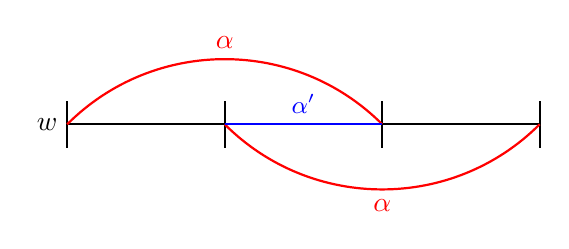
\begin{tikzpicture}
      \foreach \x in {0,2,4,6}{
        \coordinate (P\x) at (\x,0);
        \draw[thick] (P\x) -- ++(0,-0.3);
        \draw[thick] (P\x) -- ++(0,0.3);
      }
      
      \draw[thick] (P0) -- (P6);

      \node[left] at (P0) {\(w\)};
      \draw[thick, red, bend left=45] (P0) to node[midway, above, red] {\(\alpha\)} (P4);
      \draw[thick, red,bend right=45] (P2) to node[midway, below, red] {\(\alpha\)} (P6);

      \draw[thick, blue] (P2) to node[midway, above, blue,font=\small]{\(\alpha'\)} (P4);
    \end{tikzpicture}
  \end{figure}
  Infatti, essendo che \(\abs{\alpha} > \frac{\abs{w}}{2}\) e \(\alpha\) è sia prefisso che suffisso di \(w\), necessariamente deve esistere una sovrapposizione \(\alpha'\) non vuota.
  Inoltre \(\alpha'\neq\alpha\), poiché essendo \(\alpha\) bordo dev'essere prefisso e suffisso proprio di \(w\) e l'unico caso in cui \(\alpha' = \alpha\) è quello in cui le due occorrenze di \(\alpha\) coincidono, portando a \(\alpha = w\).
  In più, com'è evidente dalla figura, \(\alpha'\) è sia prefisso che suffisso di \(\alpha\), dunque è un bordo di \(\alpha\).

  Ovviamente, un bordo di \(\alpha\) è anche un bordo di \(w\), poiché è sia prefisso di un prefisso di \(w\) che suffisso di un suffisso di \(w\).
  Inoltre, si ha che \(\abs{\alpha'} < \abs{\alpha}\), dunque, ripetendo questo ragionamento, si arriva necessariamente a un bordo \(\beta\) di \(w\) tale che \(\abs{\beta} \leq \frac{\abs{w}}{2}\).
\end{proof}

Questa proposizione fa si che sia sufficiente analizzare prefissi e suffissi fino alla metà della lunghezza di una parola per scoprire se essa ammette bordi.

\begin{lemma}[label=lem:marcus-schutzenberger]{Marcus-Schützenberger}
  Sia \(X \subseteq A^+\) completo e non denso e \(\mu\) una distribuzione positiva su \(A\).
  Allora \(\mu(X) \geq 1\).
\end{lemma}
\begin{proof}
  Dato che \(X\) è non denso, esiste una parola \(w \in A^*\) che non si completa in \(X\).
  Sia \(y \in A^*\) qualsiasi.
  Essendo che \(X\) è completo, la parola \(wyw\) si completa in \(X^*\), ovvero:
  \[\exists \lambda,\rho \in A^*\st \lambda w y w \rho  = x_1x_2\ldots x_n\in X^*\]
  \begin{figure}[H]
    \centering
    \begin{tikzpicture}
      \foreach \x in {0,2,4,6,8,10}{
        \coordinate (P\x) at (\x,0);
        \draw[thick] (P\x) -- ++(0,-0.3);
        \draw[thick] (P\x) -- ++(0,0.3);
      }
     
      \draw[thick] (P0) -- (P10);

      \node at ($(P0)!0.5!(P2)$) [below] {\(\lambda\)};
      \node at ($(P2)!0.5!(P4)$) [below] {\(w\)};
      \node at ($(P4)!0.5!(P6)$) [below] {\(y\)};
      \node at ($(P6)!0.5!(P8)$) [below] {\(w\)};
      \node at ($(P8)!0.5!(P10)$) [below] {\(\rho\)};

      \draw[thick, red, bend left=45] (P0) to node[midway, above, red] {\(x_1\)} (1,0);
      \draw[thick, red, bend left=45] (1,0) to node[midway, above, red] {\(x_2\)} (3,0);
      \draw[thick, red, bend left=45] (3,0) to node[midway, above, red] {\(x_i\)} (4.5,0);
      \draw[thick, red, bend left=45] (4.5,0) to (5.5,0);
      \draw[thick, red, bend left=45] (5.5,0) to  node[midway, above, red] {\(x_j\)} (6.5,0);
      \draw[thick, red, bend left=45] (6.5,0) to (7,0);
      \draw[thick, red, bend left=45] (7,0) to (9,0);
      \draw[thick, red, bend left=45] (9,0) to node[midway, above, red] {\(x_n\)} (P10);
    \end{tikzpicture}
  \end{figure}

  Tale concatenazione è ottenibile come concatenazione di parole di \(X\), ma essendo che \(w\) non si completa in \(X\), nessuna delle occorrenze di \(w\) può essere contenuta interamente in una parola di \(X\).
  Dunque entrambe le occorrenze di \(w\) contengono almeno una \qi{linea di parsing} tra due parole di \(X\), ovvero un punto in cui termina una parola della fattorizzazione e inizia la seguente.
  Formalmente, esistono \(i,j \st 1 \leq i \leq j \leq n\) tali che \(x_i\) inizia all'interno della prima occorrenza di \(w\) e \(x_j\) termina all'interno della seconda occorrenza di \(w\).

  Dunque \(wyw \in Pref(w)\cdot X^* \cdot Suff(w)\), poiché la parte iniziale fino alla fine di \(x_i\) è un prefisso di \(w\), la parte finale da inizio di \(x_j\) alla fine è un suffisso di \(w\), e la parte centrale è ottenuta concatenando parole di \(X\).
  Essendo che \(y\) è arbitrario, si ha che \(\set{w}A^*\set{w} \subseteq Pref(w)\cdot X^* \cdot Suff(w)\)
  Dalle Proposizioni~\ref{prop:distribution_monotonicity} e~\ref{prop:distribution_distributivity_over_product}, segue che:
  \[\mu(\set{w}A^*\set{w}) \leq \mu(Pref(w)\cdot X^* \cdot Suff(w)) \leq \mu(Pref(w))\cdot \mu(X^*)\cdot \mu(Suff(w))\]
  Inoltre il prodotto \(\set{w}\times A^* \times \set{w}\) è chiaramente non ambiguo, dunque dal viceversa della \Cref{prop:distribution_distributivity_over_product}, segue che:
  \[{\mu(\set{w})}^2\mu(A^*)=\mu(\set{w}A^*\set{w}) \leq \mu(Pref(w)\cdot X^* \cdot Suff(w)) \leq \mu(Pref(w))\cdot \mu(X^*)\cdot \mu(Suff(w))\]

  Essendo che \(\mu\) è positiva, si ha che \({\mu(\set{w})}^2 > 0\), e dalla \Cref{prop:A_power_mesure_1} sappiamo che \(\mu(A^*) = \infty\).
  Dunque, per la disuguaglianza precedente, abbiamo che:
  \[\infty = {\mu(\set{w})}^2\mu(A^*) \leq \mu(Pref(w))\cdot \mu(X^*)\cdot \mu(Suff(w))\]
  E di conseguenza \(\mu(Pref(w))\cdot \mu(X^*)\cdot \mu(Suff(w)) = \infty\).
  Me essendo \(Pref(w)\) e \(Suff(w)\) finiti la loro misura è finita, dunque deve essere \(\mu(X^*) = \infty\).
  Abbiamo dunque dalla \Cref{prop:dist_union_leq_sum_dist} che:
  \[\infty = \mu(X^*) = \mu(\bigcup_{k \geq 0}^{\infty} X^k) \leq \sum_{k \geq 0}^{\infty} \mu(X^k)\]
  Inoltre dalla \Cref{prop:distribution_distributivity_over_product}, segue che:
  \[\infty = \mu(X^*) = \mu(\bigcup_{k \geq 0}^{\infty} X^k) \leq \sum_{k \geq 0}^{\infty} \mu(X^k)\leq \sum_{k \geq 0}^{\infty} {\mu(X)}^k\]
  In particolare, l'ultimo membro è una serie geometrica, che essendo maggiore o uguale a \(\infty\) diverge.
  Per far si che la serie geometrica diverga, è necessario che il suo ragione (in questo caso \(\mu(X)\)) sia maggiore o uguale a \(1\).
  Da cui segue che \(\mu(X) \geq 1\).
\end{proof}

\begin{warning}{}
  Il lemma che segue è stato presentato nel materiale originale come parte della dimostrazione del \Cref{thm:schutz_maximality_completeness}, ma è riportato separatamente qui per rendere la dimostrazione più leggibile.
\end{warning}

\begin{lemma}[label=lem:code_not_complete_boredless_word]{}
  Sia \(X \subseteq A^+\) codice non completo, con \(\# A \geq 2\).
  Allora esiste una parola \(y \in A^*\) senza bordi che non si completa in \(X^*\).
\end{lemma}
\begin{proof}
  Essendo che \(X\) non è completo, esiste una parola \(z \in A^*\) che non si completa in \(X^*\).
  Se tale parola non ha bordi, allora abbiamo finito.
  Altrimenti, supponiamo che \(z\) abbia bordi e inizi per \(a \in A\).
  Sia dunque \(b \in A\setminus\set{a}\) (esistenza garantita dal fatto che \(\# A \geq 2\)) e consideriamo la parola \(y = zb^{\abs{z}}\).
  Tale parola non può completarsi in \(X^*\), poiché se così fosse, essendo che \(z\) è prefisso di \(y\), anche \(z\) si completerebbe in \(X^*\), contraddicendo l'ipotesi.
  Inoltre, \(y\) non può avere bordi, poiché dalla Preposizione~\ref{prop:if_border_exists_border_half_length} per valutare se \(y\) ha bordi è sufficiente considerare i prefissi e suffissi di lunghezza al più \(\frac{\abs{y}}{2} = \abs{z}\).
  Si ha dunque che tutti i prefissi di \(y\) iniziano per \(a\) (poiché la prima metà di \(y\) è proprio \(z\)), mentre tutti i suffissi di lunghezza al più \(\abs{z}\) iniziano per \(b\) (poiché la seconda metà di \(y\) è composta di sole \(b\)), dunque non possono coincidere, e di conseguenza \(y\) non ha bordi.
\end{proof}

A questo punto siamo in grado di dimostrare il Teorema di Schützenberger~\ref{thm:schutz_maximality_completeness}.
\begin{proof}[Dimostrazione di~\ref{thm:schutz_maximality_completeness}]
  \begin{enumerate}
    \item Per dimostrare che se \(X\) è massimale allora è completo, procediamo per contrapposizione, ovvero assumendo che \(X\) non sia completo e mostrando che in tal caso non può essere massimale.
      Iniziamo escludendo il caso banale in cui \(\# A = 1\). In questo casi infatti, tutti i codici possibili sono singleton, poiché ogni altro insieme di parole porta a parole con plurime fattorizzazioni\footnote{Si prenda ad esempio \(Z = \set{a^k,a^h}\). In tal caso \(a^{h+k} = a^h a^k = a^k a^h\)}.
      Di conseguenza tutti i codici sono massimali, e sono inoltre anche completi, poiché ogni parola \(a^m\) si completa in \(X = \set{a^h}\) aggiungendo a \(a^m\) tante \(a\) fino a raggiungere un multiplo di \(h\).

      Sia dunque \(\# A \geq 2\) e sia \(y \in A^*\) che non si completa in \(X^*\) (esistenza garantita dal fatto che \(X\) è assunto non completo).
      Possiamo scegliere senza perdita di generalità \(y\) senza bordi dal \Cref{lem:code_not_complete_boredless_word}.

      Consideriamo dunque l'insieme \(Y=X\cup\set{y}\). Se tale insieme fosse codice, si avrebbe che \(X\) non è massimale, come volevamo dimostrare.
      Supponiamo dunque per assurdo che non lo sia.
      Allora esiste una parola di \(Y^*\) con multipla fattorizzazione, ovvero esistono \(y_1,y_2,\ldots y_m,y_1',y_2',\ldots,y_n' \in Y\) tali che \(y_1y_2\ldots y_m = y_1y_2\ldots y_n'\), con \(y_1\neq y_1'\).
      Tra queste parole deve necessariamente esserci almeno una occorrenza di \(y\), poiché altrimenti tale parola apparterrebbe a \(X^*\), contraddicendo l'ipotesi che \(X\) è codice.
      Inoltre, essendo che \(y\) non si completa in \(X^*\), dev'esserci almeno un occorrenza di \(y\) in entrambe le fattorizzazioni.
      Questo poiché se fosse presente solo in una delle due, si potrebbe completare \(y\) in \(X^*\) prendendo la parola in cui è presente \(y\) come completamento e l'altro membro della uguaglianza come parola di \(X^*\).
      Dunque \(\exists i,j \st y_i=y_j'=y\). Scegliamo senza perdita di generalità \(i\) e \(j\) minimi con tale proprietà.

      Analizziamo dunque per casi i possibili posizionamenti delle due occorrenze di \(y\) nelle due fattorizzazione sovrapposte:
      \begin{description}
        \item[Le due occorrenze di \(y\) non hanno sovrapposizione]
          In questo caso, è possibile rappresentare le due fattorizzazioni come segue:
          \begin{figure}[H]
            \centering
            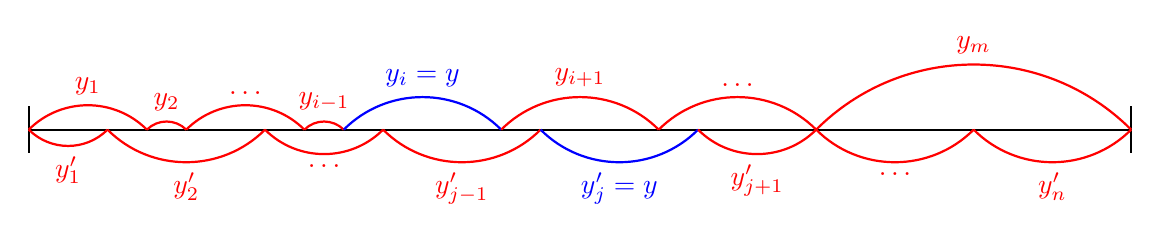
\begin{tikzpicture}
              \foreach \x in {0,2,4,6,8,10,12,14}{
                \coordinate (P\x) at (\x,0);
              }
             
              \draw[thick] (P0) -- ++(0,-0.3);
              \draw[thick] (P0) -- ++(0,0.3);
              \draw[thick] (P14) -- ++(0,-0.3);
              \draw[thick] (P14) -- ++(0,0.3);
              \draw[thick] (P0) -- (P14);

              \draw[thick, red, bend left=45] (P0) to node[midway, above, red] {\(y_1\)} (1.5,0);
              \draw[thick, red, bend left=45] (1.5,0) to node[midway, above, red] {\(y_2\)} (2,0);
              \draw[thick, red, bend left=45] (2,0) to node[midway, above, red] {\(\ldots\)} (3.5,0);
              \draw[thick, red, bend left=45] (3.5,0) to node[midway, above, red] {\(y_{i-1}\)} (4,0);
              \draw[thick, blue, bend left=45] (4,0) to node[midway, above, blue] {\(y_i = y\)} (6,0);
              \draw[thick, red, bend left=45] (6,0) to node[midway, above, red] {\(y_{i+1}\)} (P8);
              \draw[thick, red, bend left=45] (P8) to node[midway, above, red] {\(\ldots\)} (P10);
              \draw[thick, red, bend left=45] (P10) to node[midway, above, red] {\(y_m\)} (P14);

              \draw[thick, red, bend right=45] (P0) to node[midway, below, red] {\(y_1'\)} (1,0);
              \draw[thick, red, bend right=45] (1,0) to node[midway, below, red] {\(y_2'\)} (3,0);
              \draw[thick, red, bend right=45] (3,0) to node[midway, below, red] {\(\ldots\)} (4.5,0);
              \draw[thick, red, bend right=45] (4.5,0) to node[midway, below, red] {\(y_{j-1}'\)} (6.5,0);
              \draw[thick, blue, bend right=45] (6.5,0) to node[midway, below, blue] {\(y_j' = y\)} (8.5,0);
              \draw[thick, red, bend right=45] (8.5,0) to node[midway, below, red] {\(y_{j+1}'\)} (P10);
              \draw[thick, red, bend right=45] (P10) to node[midway, below, red] {\(\ldots\)} (P12);
              \draw[thick, red, bend right=45] (P12) to node[midway, below, red] {\(y_n'\)} (P14);
            \end{tikzpicture}
          \end{figure}
          In questo caso però, sarebbe possibile completare \(y\) in \(X^*\), poiché la parola \(y_1'y_2'\ldots y_{j-1}'\) appartiene a \(X^*\) per minimalità di \(j\), e contiene \(y\) come sottoparola. Assurdo!
          \item[Le due occorrenze di \(y\) hanno sovrapposizione parziale]
          In questo caso, è possibile rappresentare le due fattorizzazioni come segue:
          \begin{figure}[H]
            \centering
            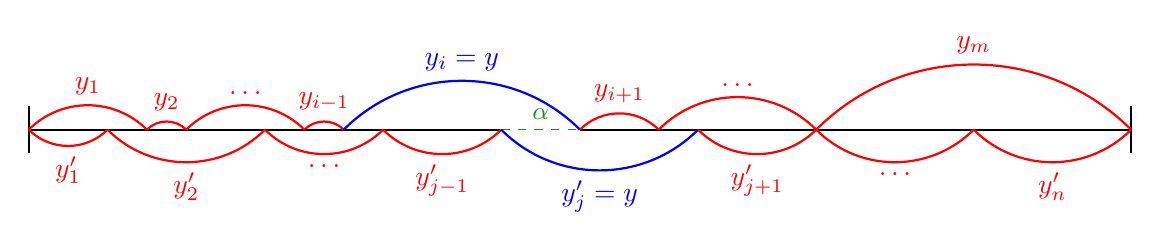
\begin{tikzpicture}
              \foreach \x in {0,2,4,6,8,10,12,14}{
                \coordinate (P\x) at (\x,0);
              }
             
              \draw[thick] (P0) -- ++(0,-0.3);
              \draw[thick] (P0) -- ++(0,0.3);
              \draw[thick] (P14) -- ++(0,-0.3);
              \draw[thick] (P14) -- ++(0,0.3);
              \draw[thick] (P0) -- (P14);

              \draw[thick, white] (6,0) to (7,0);
              \draw[dashed, ForestGreen] (6,0) to node[midway, above=0.01pt, ForestGreen,font=\small]{\(\alpha\)} (7,0);

              \draw[thick, red, bend left=45] (P0) to node[midway, above, red] {\(y_1\)} (1.5,0);
              \draw[thick, red, bend left=45] (1.5,0) to node[midway, above, red] {\(y_2\)} (2,0);
              \draw[thick, red, bend left=45] (2,0) to node[midway, above, red] {\(\ldots\)} (3.5,0);
              \draw[thick, red, bend left=45] (3.5,0) to node[midway, above, red] {\(y_{i-1}\)} (4,0);
              \draw[thick, blue, bend left=45] (4,0) to node[midway, above, blue] {\(y_i = y\)} (7,0);
              \draw[thick, red, bend left=45] (7,0) to node[midway, above, red] {\(y_{i+1}\)} (P8);
              \draw[thick, red, bend left=45] (P8) to node[midway, above, red] {\(\ldots\)} (P10);
              \draw[thick, red, bend left=45] (P10) to node[midway, above, red] {\(y_m\)} (P14);

              \draw[thick, red, bend right=45] (P0) to node[midway, below, red] {\(y_1'\)} (1,0);
              \draw[thick, red, bend right=45] (1,0) to node[midway, below, red] {\(y_2'\)} (3,0);
              \draw[thick, red, bend right=45] (3,0) to node[midway, below, red] {\(\ldots\)} (4.5,0);
              \draw[thick, red, bend right=45] (4.5,0) to node[midway, below, red] {\(y_{j-1}'\)} (6,0);
              \draw[thick, blue, bend right=45] (6,0) to node[midway, below, blue] {\(y_j' = y\)} (8.5,0);
              \draw[thick, red, bend right=45] (8.5,0) to node[midway, below, red] {\(y_{j+1}'\)} (P10);
              \draw[thick, red, bend right=45] (P10) to node[midway, below, red] {\(\ldots\)} (P12);
              \draw[thick, red, bend right=45] (P12) to node[midway, below, red] {\(y_n'\)} (P14);

            \end{tikzpicture}
          \end{figure}
          Tale sovrapposizione è indicata in verde nella figura come \(\alpha\).
          Essendo però \(\alpha\) sia suffisso di \(y\) (essendo parte della occorrenza \(i\) di \(y\)) che prefisso di \(y\) (essendo parte della occorrenza \(j\) di \(y\)), e non essendo \(\alpha = y\) (poiché le due occorrenze di \(y\) non coincidono), si ha che \(\alpha\) è un bordo di \(y\), contraddicendo l'ipotesi che \(y\) non abbia bordi. Assurdo!
        \item[Le due occorrenze di \(y\) sono allineate]
          Infine, consideriamo il caso in cui le due occorrenze di \(y\) siano allineate, ovvero:
          \begin{figure}[H]
            \centering
            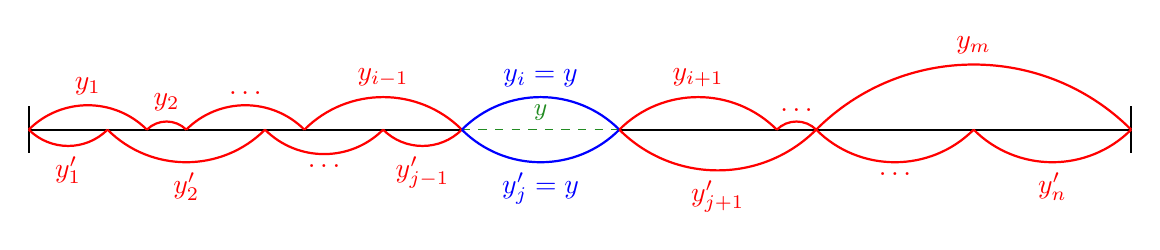
\begin{tikzpicture}
              \foreach \x in {0,2,4,6,8,10,12,14}{
                \coordinate (P\x) at (\x,0);
              }
             
              \draw[thick] (P0) -- ++(0,-0.3);
              \draw[thick] (P0) -- ++(0,0.3);
              \draw[thick] (P14) -- ++(0,-0.3);
              \draw[thick] (P14) -- ++(0,0.3);
              \draw[thick] (P0) -- (P14);

              \draw[thick, white] (5.5,0) to (7.5,0);
              \draw[dashed, ForestGreen] (5.5,0) to node[midway, above=0.01pt, ForestGreen,font=\small]{\(y\)} (7.5,0);

              \draw[thick, red, bend left=45] (P0) to node[midway, above, red] {\(y_1\)} (1.5,0);
              \draw[thick, red, bend left=45] (1.5,0) to node[midway, above, red] {\(y_2\)} (2,0);
              \draw[thick, red, bend left=45] (2,0) to node[midway, above, red] {\(\ldots\)} (3.5,0);
              \draw[thick, red, bend left=45] (3.5,0) to node[midway, above, red] {\(y_{i-1}\)} (5.5,0);
              \draw[thick, blue, bend left=45] (5.5,0) to node[midway, above, blue] {\(y_i = y\)} (7.5,0);
              \draw[thick, red, bend left=45] (7.5,0) to node[midway, above, red] {\(y_{i+1}\)} (9.5,0);
              \draw[thick, red, bend left=45] (9.5,0) to node[midway, above, red] {\(\ldots\)} (P10);
              \draw[thick, red, bend left=45] (P10) to node[midway, above, red] {\(y_m\)} (P14);

              \draw[thick, red, bend right=45] (P0) to node[midway, below, red] {\(y_1'\)} (1,0);
              \draw[thick, red, bend right=45] (1,0) to node[midway, below, red] {\(y_2'\)} (3,0);
              \draw[thick, red, bend right=45] (3,0) to node[midway, below, red] {\(\ldots\)} (4.5,0);
              \draw[thick, red, bend right=45] (4.5,0) to node[midway, below, red] {\(y_{j-1}'\)} (5.5,0);
              \draw[thick, blue, bend right=45] (5.5,0) to node[midway, below, blue] {\(y_j' = y\)} (7.5,0);
              \draw[thick, red, bend right=45] (7.5,0) to node[midway, below, red] {\(y_{j+1}'\)} (P10);
              \draw[thick, red, bend right=45] (P10) to node[midway, below, red] {\(\ldots\)} (P12);
              \draw[thick, red, bend right=45] (P12) to node[midway, below, red] {\(y_n'\)} (P14);

            \end{tikzpicture}
          \end{figure}
          In tale situazione però si avrebbe che \(y_1y_2\ldots y_{i+1} = y_1'y_2'\ldots y_{j-1}'\) è una doppia fattorizzazione di una parola ottenuta concatenando parole di \(X\), dalla minimalità di \(i\) e \(j\). Dunque questo contraddice l'ipotesi che \(X\) sia codice. Assurdo!
      \end{description}
      L'assunzione dunque che esista una doppia fattorizzazione in \(Y\), e che quindi non sia codice, porta a una contraddizione in ogni possibile caso.
      Di conseguenza, dato \(X\) non completo, è sempre possibile costruire un sovrainsieme \(Y\) che è ancora codice, mostrando che \(X\) non è massimale.
      Ergo, per contrapposizione, se \(X\) è massimale allora è completo.
    \item In questo caso, sappiamo per ipotesi che \(X\) è completo e non denso.
      Dunque presa \(\mu\) distribuzione positiva su \(A\), dal \Cref{lem:marcus-schutzenberger} sappiamo che \(\mu(X) \geq 1\).
      D'altra parte, dal \Cref{thm:kraft-mcmillan}, sappiamo che \(\mu(X) \leq 1\), poiché \(X\) è codice.
      Dunque, si ha che \(\mu(X) = 1\). Come visto in precedenza, ciò implica che \(X\) è massimale.
  \end{enumerate}
\end{proof}

\begin{note}{}
  L'ipotesi \emph{non denso} nel secondo punto del \Cref{thm:schutz_maximality_completeness} è necessaria. Infatti il codice \(Z = \{a^{|u|+1}bu | u \in {\{a,b\}}^*\}\) è un codice denso (e quindi completo), ma non massimale.
  Infatti \(Z\cup\{b\}\) è ancora un codice (prefisso).
\end{note}

Un diretto corollario del Teorema di Schützenberger è il seguente:
\begin{corollary}
  Sia \(X \subseteq A^+\) codice non denso. Allora le seguenti affermazioni sono equivalenti:
  \begin{enumerate}
    \item \(X\) è massimale
    \item \(X\) è completo
    \item \(\forall \mu\) distribuzione positiva su \(A\): \(\mu(X) = 1\)
    \item \(\exists \mu\) distribuzione positiva su \(A\): \(\mu(X) = 1\)
  \end{enumerate}
\end{corollary}
\begin{proof}
  Si ha che \(1 \iff 2\) per il punto \(1\) del \Cref{thm:schutz_maximality_completeness}, \(2 \implies 3\) viene dalla dimostrazione del punto \(2\) del \Cref{thm:schutz_maximality_completeness} per via della massimalità, \(3 \implies 4\) è banale e \(4 \implies 1\) è stato più volte dimostrato precedentemente.
\end{proof}

Vediamo dunque alcune proposizioni che seguono dai risultati appena dimostrati.

\begin{proposition}{}
  Sia \(X\subseteq A^*\) finito e completo, e \(\mu\) distribuzione positiva su \(A\) tale che \(\mu(X) = 1\). Allora \(X\) è un codice (massimale).
\end{proposition}

\begin{proof}
  \(\forall n \geq 1, X^n\) è completo. Infatti se \(w\) si completa in \(X^*\) allora si completa anche in \({(X^n)}^*\)
  Essendo \(X\) finito, anche \(X^n\) è finito, e di conseguenza è anche non denso. Dunque per il \Cref{lem:marcus-schutzenberger} si ha che:
  \[1\leq \mu(X^n) \leq {\mu(X)}^n = 1^n = 1\]
  Quindi \(\forall n \geq 1: \mu(X^n) = 1 = {\mu(X)}^n\).
  Di conseguenza, per il viceversa della \Cref{prop:code_implies_equal_mesures_of_powers} si ha che \(X\) è un codice.
  Essendo inoltre a codice con misura \(1\), è massimale.
\end{proof}



\begin{proposition}{}
  Sia \(X \subseteq A^*\) finito e completo. Allora \(\forall a \in A \exists n \geq 1 : a^n \in X\). Tale \(n\) è unico se \(X\) è un codice.
\end{proposition}
\begin{proof}
  Essendo \(X\) finito esiste una lunghezza di parola massima.
  Sia dunque \(L = \max_{x \in X}\abs{x}\) e \(a \in A\).
  Essendo \(X\) completo, \(a^{2L}\) si completa in \(X^*\), quindi esistono \(\lambda, \rho \in A^*: \lambda a^{2L} \rho \in X^*\).
  \begin{figure}[H]
    \centering
    \begin{tikzpicture}
      \foreach \x in {0,2,4,6,8,10}{
        \coordinate (P\x) at (\x,0);
      }
      
      \draw[thick] (P0) -- ++(0,-0.3);
      \draw[thick] (P0) -- ++(0,0.3);
      \draw[thick] (P2) -- ++(0,-0.3);
      \draw[thick] (P2) -- ++(0,0.3);
      \draw[thick] (P8) -- ++(0,-0.3);
      \draw[thick] (P8) -- ++(0,0.3);
      \draw[thick] (P10) -- ++(0,-0.3);
      \draw[thick] (P10) -- ++(0,0.3);
      \draw[thick] (P0) -- (P10);

      \node at ($(P0)!0.5!(P2)$) [above] {\(\lambda\)};
      \node at ($(P2)!0.5!(P8)$) [above] {\(a^{2n}\)};
      \node at ($(P8)!0.5!(P10)$) [above] {\(\rho\)};

      \draw[thick, red, bend right=45] (P0) to node[midway, below, red] {\(x_1\)} (1,0);
      \draw[thick, red, bend right=45] (1,0) to node[midway, below, red] {\(x_2\)} (3,0);
      \draw[thick, red, bend right=45] (3,0) to node[midway, below, red] {\(\ldots\)} (4.5,0);
      \draw[thick, red, bend right=45] (4.5,0) to node[midway, below, red] {\(x_i\)} (5.5,0);
      \draw[thick, red, bend right=45] (5.5,0) to node[midway, below, red] {\(\ldots\)} (7.5,0);
      \draw[thick, red, bend right=45] (7.5,0) to node[midway, below, red] {\(x_m\)} (P10);

    \end{tikzpicture}
  \end{figure}
  Essendo che ogni parola in \(X\) ha lunghezza al più \(L\), esiste un \(x_i\) della fattorizzazione di \(\lambda a^{2L} \rho\) sottoparola propria di \(a^{2L}\).
  Non fosse così si avrebbero due parole \(x_i,x_{i+1}\in X\) che composte contengono propriamente \(a^{2L}\) e che iniziano e finiscono rispettivamente prima e dopo \(a^{2L}\), ottenendo una rappresentazione di questo tipo:
    \begin{figure}[H]
    \centering
    \begin{tikzpicture}
      \foreach \x in {0,2,4,6,8,10}{
        \coordinate (P\x) at (\x,0);
      }
      
      \draw[thick] (P0) -- ++(0,-0.3);
      \draw[thick] (P0) -- ++(0,0.3);
      \draw[thick] (P2) -- ++(0,-0.3);
      \draw[thick] (P2) -- ++(0,0.3);
      \draw[thick] (P8) -- ++(0,-0.3);
      \draw[thick] (P8) -- ++(0,0.3);
      \draw[thick] (P10) -- ++(0,-0.3);
      \draw[thick] (P10) -- ++(0,0.3);
      \draw[thick] (P0) -- (P10);

      \node at ($(P0)!0.5!(P2)$) [above] {\(\lambda\)};
      \node at ($(P2)!0.5!(P8)$) [above] {\(a^{2n}\)};
      \node at ($(P8)!0.5!(P10)$) [above] {\(\rho\)};

      \draw[thick, red, bend right=45] (P0) to node[midway, below, red] {\(x_1\)} (0.5,0);
      \draw[thick, red, bend right=45] (0.5,0) to node[midway, below, red] {\(x_2\)} (1,0);
      \draw[thick, red, bend right=45] (1,0) to node[midway, below, red] {\(\ldots\)} (1.5,0);
      \draw[thick, red, bend right=45] (1.5,0) to node[midway, below, red] {\(x_i\)} (5,0);
      \draw[thick, red, bend right=45] (5,0) to node[midway, below, red] {\(x_{i+1}\)} (8.5,0);
      \draw[thick, red, bend right=45] (8.5,0) to node[midway, below, red] {\(\ldots\)} (9,0);
      \draw[thick, red, bend right=45] (9,0) to node[midway, below, red] {\(x_m\)} (P10);

    \end{tikzpicture}
  \end{figure}
  Ma in questo scenario, si avrebbe che necessariamente \(\abs{x_i x_{i+1}} = \abs{x_i} + \abs{x_{i+1}} > 2L\), implicando che almeno una delle due parole ha lunghezza maggiore di \(L\), assurdo.
  
  Da ciò segue che tale \(x_i\) è della forma \(a^n\). Se \(X\) è codice questo \(n\) è unico poiché se esistesse \(m\neq n\) tale che \(a^m \in X\), allora la parola \(a^{n+m}\) avrebbe due fattorizzazioni distinte in \(X^*\) portando all'assurdo.
\end{proof}

\begin{definition}{Completamento di un codice}
  Sia \(X \subseteq A^*\) un codice.
  Un \emph{completamento} di \(X\) è un codice \(Y \supseteq X\) sullo stesso alfabeto che sia massimale.

  In altre parole, un completamento di un codice \(X\) è un sovrainsieme massimale di \(X\) che sia ancora un codice.
\end{definition}
Da questa definizione sorgono alcune domande riguardo la completabilità dei codici:
\begin{enumerate}
  \item Dato un codice \(X\) qualsiasi, esiste sempre un completamento?
    Tale quesito ha risposta affermativa, e ne vedremo la dimostrazione più avanti.
  \item Dato un codice \(X\) finito, esiste sempre un completamento finito?
    In questo caso la risposta è negativa.
    Un esempio noto fornito da Markov ha mostrato che dato \(A = \set{a,b}\), il codice \(X = \set{a^5,ab,ba^2,b}\) non ha completamenti finiti.
  \item A questo punto, \emph{quali} codici finiti ammettono completamento finito?
    In generale, la caratterizzazione completa è un problema aperto, ma:
    \begin{itemize}
      \item I codici finiti prefissi ammettono sempre completamenti finiti.
        Caso particolare di questo caso qualsiasi codice finito con cardinalità \(1\) ammette sempre completamento finito.
      \item Se \(\#X = 2\), allora \(X\) ammette un completamento finito, dimostrato da Restivo.\todo{Chiedere se effettivamente questo Restivo è chi ha dimostrato}
      \item Se \(\#X \geq 4\), in generale non ammette un completamento finito. Infatti l'esempio di Markov ha cardinalità \(4\).
      \item Se \(\#X = 3\), il problema è aperto.
    \end{itemize}
\end{enumerate}


Vediamo dunque la dimostrazione dell'esistenza di un completamento per ogni codice citato in precedenza.
\begin{proposition}{}
  Sia \(X \subseteq A^*\) codice. Allora esiste un completamento di \(X\).
\end{proposition}
\begin{proof}
  Se \(X\) è massimale, allora \(X = X_0\) è un completamento di sé stesso.
  Altrimenti, esiste \(w_1 \in A^*\setminus X\) di lunghezza minima tale che \(X_1 = X \cup \{w_1\}\) è ancora un codice.
  Se \(X_1\) è massimale, abbiamo finito.
  In generale, se iterando questo procedimento otteniamo \(X_k = X_{k-1} \cup \set{w_k}\) massimale, abbiamo finito.
  Altrimenti, otteniamo una successione infinita di parole \(s = \set{w_n}\). Essendo però l'alfabeto finito, esistono parole in \(s\) arbitrariamente lunghe.
  Mostriamo dunque che \(Y = \bigcup_{k = 0}^{\infty} X_k\) è un codice massimale.
  È codice poiché se avessimo una doppia fattorizzazione \(y_1 y_2 \cdots y_n = y_1' y_2' \cdots y_m'\) avremmo che ogni \(y_i\) e \(y_j'\) appartengono a qualche \(X_k\). Essendo che \(X_0 \subseteq X_1 \subseteq X_2 \subseteq \cdots\), esiste \(n\) tale che tutti i \(y_i\) e \(y_j'\) appartengono a \(X_n\). Ma allora avremmo una doppia fattorizzazione in \(X_n\), assurdo.
  Per quanto riguarda la massimalità, se avessimo \(w \in A^* \setminus Y\) tale che \(Y \cup \{w\}\) è ancora un codice, allora esisterebbe \(m\) tale che \(\abs{w_m} > \abs{w}\), poiché aggiungendo parole all'infinito dovrò necessariamente saturare tutte le parole di lunghezza minore di una certa soglia.
  
  Ma allora \(X_{m-1} \cup \set{w}\subseteq Y \cup \set{w}\) sarebbe ancora codice, contraddicendo la minimalità di \(w_m\).
\end{proof}

Con quest'ultimo risultato, si conclude la trattazione delle proprietà algebriche dei codici, che ci serviranno come presupposti teorici per la trattazione della codifica di sorgente nel capitolo successivo, che si addentrerà maggiormente sugli aspetti legati alla teoria dell'informazione.





% Dopo questa sezione (che corrisponde alla lezione 6 del 6 ottobre) siamo "in pari" col file draft, nel senso che quello che viene dopo è già scritto nel file draft e va solo ripulito.
% Dopo tale file poi ci sono i tuoi appunti in obsidian da trascrivere delle lezioni in cui ero in finlandia.
% Fatto ciò siamo in pari
\chapter{Codifica di Sorgente}

Ci inoltriamo finalmente nel cuore della teoria dell'informazione, ovvero la codifica di sorgente.

\section{Sorgenti e Codifica}

\begin{definition}{Sorgente (discreta e a memoria zero)}
  Chiamiamo \keyword{Sorgente discreta e a memoria zero} una variabile aleatoria discreta, identificabile come una coppia \(S = (\SCal,p)\), con \(\SCal\) alfabeto sorgente, ovvero l'insieme dei simboli che la sorgente può emettere,
  ovvero i valori che la variabile aleatoria può assumere, e \(p\) distribuzione su \(\SCal\).
\end{definition}

\begin{definition}{Codifica}
  Definiamo \keyword{codifica} un morfismo iniettivo \(\varphi: \SCal^* \to A^*\) con \(A\) alfabeto (di codice).
  Il \keyword{codice} relativo a questa codifica è \(X = \varphi(\SCal)\), ovvero l'immagine di \(\SCal\) sotto \(\varphi\).
\end{definition}

\todo{Mi ricordo che disse che la ridotta alla base è biettiva}
\todo{Inoltre mi pare si parlasse solo di alfabeti finiti, mi sbaglio?}

\begin{definition}{Costo di una codifica}
  Data una sorgente \(S = (\SCal,p)\) e una codifica \(\varphi: \SCal^* \to A^*\) con codice \(X = \varphi(\SCal)\), definiamo il \keyword{costo} di \(\varphi\) la quantità:
  \[c(X,\varphi) = \sum_{s \in \SCal} p(s) \abs{\varphi(s)}\]
  ovvero la media pesata sulla distribuzione \(p\) delle lunghezze delle parole codificate.
  Il \keyword{costo assoluto} di un codice \(X\) sarà
  \[c(X) = \min_{\varphi: \varphi(\SCal) \leftrightarrow  X} c(X,\varphi)\]
\end{definition}


\begin{example}[label=ex:codifica]{}
  Sia \(\SCal = \set{s_1,s_2,s_3}\), \(A = \set{a,b}\), \(X = \set{a,ba,bb}\).
  Se \(p(s_1) = 1/2, p(s_2) = p(s_3) = 1/4\), e inoltre \(\varphi(s_1) = ba, \varphi(s_2) = a, \varphi(s_3) = bb\), si ha che
    \[c(X,\varphi) = \frac{7}{4} > c(X) = \frac{3}{2}\]
\end{example}

Da questo esempio è possibile trarne una regola generale.

\begin{proposition}{}
  Sia \(S\) sorgente, \(X\) codice su \(A\) \emph{adattato}\footnote{Ovvero tale che esiste un morfismo biettivo tra \(\S\) e \(X\). In questo caso mediante \(\varphi\) si intende che un morfismo biettivo è \(\varphi_{|_{\SCal}}\)} a \(S\) mediante \(\varphi\).
  Allora \(c(X) = c(X,\varphi)\) se e solo se
    \[\forall s,s' \in \SCal, p(s) < p(s') \implies \abs{\varphi(s)} < \abs{\varphi(s')} \]
\end{proposition}

\begin{proof}
  La dimostrazione è abbastanza intuitiva, in quanto la proposizione è l'unico modo per minimizzare la somma pesata delle lunghezze.
\end{proof}

In altre parole, per minimizzare il costo di una codifica, i simboli più probabili devono essere codificati con parole più corte.

\begin{definition}{Codice ottimale}
  Diremo che \(X\) è un \keyword{codice ottimale} per la sorgente \(S\) se, per ogni codice \(Z\) sullo stesso alfabeto e di cardinalità \(\# X = \# \SCal\), si ha che
  \[c(X) \leq c(Z)\]
\end{definition}

\begin{example}{}
  Data la sorgente dell'esempio~\ref{ex:codifica}, il codice \(Z = \set{aa,ba,bb}\) \textbf{non} è ottimale, poiché \(c(Z) = 2\), mentre abbiamo trovato un codice di costo inferiore nell'esempio precedente.
\end{example}

\section{Entropia di una sorgente}

\begin{definition}{Entropia di una sorgente}
  Data una sorgente \(S = (\SCal,p)\), definiamo l'\keyword{entropia} di \(S\) la quantità
  \[H(S) = -\sum_{s \in \SCal} p(s) \log\left(p(s)\right) = \sum_{s \in \SCal} p(s) \log\left(\frac{1}{p(s)}\right)\]  
\end{definition}

Tale quantità rappresenta un valore medio dell'autoinformazione (ovvero dell'incertezza) della sorgente.
La base del logaritmo non è specificata, non perché non cambi il valore di \(H(S)\), ma poiché la variazione è solo un fattore moltiplicativo costante, analogo a un cambio di unità di misura.

Corrispondentemente l'entropia (e l'informazione in generale) si misura utilizzando comunemente tre unità di misura:
\begin{itemize}
  \item \emph{hartley} (base \(10\)), prima unità di misura dell'informazione
  \item \emph{nat} (base \(e\)), utile per alcune formulazioni matematiche
  \item \emph{bit} (base \(2\)), più utilizzata al giorno d'oggi
\end{itemize}
L'entropia di \(1 bit\) è quella di una sorgente binaria uniforme:
\[H(S) = \frac{1}{2}\log_2(2) + \frac{1}{2}\log_2(2) = 1\]
Da questo momento in avanti si farà riferimento unicamente ai \(bit\) come unità di misura dell'informazione, omettendo dunque la base del logaritmo.

\begin{note}{}
  La definizione di entropia fornita non esclude la possibilità di avere \(p(s) = 0\) per qualche \(s \in \SCal\).
  In tal caso il termine della somma corrispondente a tale \(s\) non sarebbe definito. 
  Dunque si assume che il termine \(p(s)\log\left(p(s)\right) = 0\) per continuità, dato che \(\lim_{x \to 0^+} x \log\left(x\right) = 0\).

  In maniera formale, si può ridefinire l'entropia come
  \[H(S) = -\sum_{s \in \SCal} h(s)\]
  dove
  \[h(s) = \begin{cases}
              p(s) \log\left(p(s)\right) & , p(s) > 0 \\
              0 & , p(s) = 0
            \end{cases}
  \]
\end{note}

In generale si ha che \(0 \leq H(S) \leq \log\left(\#\SCal\right)\), e inoltre possibile caratterizzare tali casi limite.
Il limite inferiore è dato da:
\begin{equation}\label{eq:lower_bound_entropy}
    H(S) = 0 \iff \exists s \in \SCal: p(s) = 1
\end{equation}

Ovviamente dalla definizione di distribuzione segue che \(\forall s' \neq s: p(s') = 0\).

Mentre il limite superiore è dato da:
\begin{equation}\label{eq:upper_bound_entropy}
  H(S) = \log\left(\#\SCal\right) \iff \forall s \in \SCal: p(s) = \frac{1}{\#\SCal}
\end{equation}
Ovvero l'entropia (e quindi l'incertezza) è nulla se la sorgente è certa (emette sempre lo stesso simbolo), e massima se la sorgente è uniforme (emette tutti i simboli con la stessa probabilità).

Andiamo dunque a dimostrare tali affermazioni.

\begin{proof}[Dimostrazione di~\ref{eq:lower_bound_entropy}]
  Essendo che \(\forall s \in \SCal: 0\leq p(s) \leq 1\), abbiamo che\footnote{È denotato che \(-\infty \leq \log\left(p(s)\right)\) e non \(-\infty < \log\left(p(s)\right)\), poiché si assume \(\log\left(0\right)\) definito come \(-\infty\) per continuità.}
  \[-\infty \leq \log\left(p(s)\right) \leq 0 \iff  0 \leq -\log\left(p(s)\right) = \log\left(\frac{1}{p(s)}\right) \leq \infty\]

  Dunque \(H(S) = \sum_{s \in \SCal} p(s) \log\left(\frac{1}{p(s)}\right) = E[\log\left(\frac{1}{p(S)}\right)] \geq 0\), essendo somma pesata (o media) di quantità non negative.

  Inoltre se \(p(s) = 1\) e \(p(t) = 0 \forall t \in \SCal \setminus \set{s}\) si ha che
  \[H(S) = 1 \cdot \log\left(\frac{1}{1}\right) - \sum_{t \in \SCal \setminus \set{s}} 0 \cdot \log\left(0\right) = 0 - 0 = 0\]
  Viceversa, se \(H(S) = 0\), deve aversi che \(\forall s \in \SCal: p(s) \log\left(\frac{1}{p(s)}\right) = 0\), che può avvenire solo in due casi, ovvero \(\forall s \in \SCal p(s) = 0 \lor p(s) = 1\).
  Ma essendo che \(p\) è una distribuzione, \(\sum_{s \in \SCal} p(s) = 1\), e dunque
  \[\exists!\bar{s} \in \SCal: p(\bar{s}) = 1\]
\end{proof}

\begin{proof}[Dimostrazione di~\ref{eq:upper_bound_entropy}]
  Si può utilizzare la disuguaglianza di Gibbs.
  Tale disuguaglianza afferma che, date due distribuzioni \(p\) e \(q\) su \(\SCal\), Allora:
  \begin{equation}\label{eq:gibbs}
    \sum_{s \in \SCal} p(s) \log\left(\frac{1}{p(s)}\right) \leq -\sum_{s \in \SCal} p(s) \log\left(\frac{1}{q(s)}\right)
  \end{equation}
  Ovvero che l'entropia di \(S\) rispetto a \(p\) è minore o uguale alla media in probabilità \(p\) dell'inverso del logaritmo della probabilità secondo \(q\), e vale l'uguaglianza se e solo se \(p = q\).
  \begin{note}{}
    È importate notare che il lato destro della disuguaglianza può divergere, poiché essendo le distribuzioni diverse non è possibile definire separatamente il caso dello \(0\), poiché le due distribuzioni potrebbero essere nulle in punti diversi.
  \end{note}
  Posto \(q(s) = \frac{1}{\#\SCal}, \forall s \in \SCal\), per la disuguaglianza di Gibbs si ha che
  \[H(S) \leq \sum_{s \in \SCal} p(s) \log\left(\#\SCal\right) = \log\left(\#\SCal\right)\sum_{s \in \SCal} p(s) = \log\left(\#\SCal\right)\]
  Inoltre, per l'uguaglianza, deve aversi che \(p = q\). Dunque, essendo \(H(S)\) superiormente limitata da un valore che può assumere, tale valore è il massimo di \(H(S)\), e si ha che tale massimo è raggiunto se e solo se \(p\) è la distribuzione uniforme su \(\SCal\).
\end{proof}

Possiamo dunque arrivare a un risultato fondamentale per questo corso che lega l'entropia di una sorgente al costo di codifica, ovvero il teorema di Shannon.

\begin{theorem}{Shannon}
  Sia \(S = (\SCal,p)\) sorgente, \(A\) alfabeto di codice con \(\#\SCal = d \geq 2\) e \(X \subseteq A^+\) codice adattato a \(S\) mediante \(\varphi\).
  Allora
  \[c(X,\varphi) \geq \frac{H(S)}{\log\left(d\right)}\]
  Inoltre, vale l'uguaglianza se e solo se:
  \begin{itemize}
    \item \(X\) è massimale;
    \item \(\forall s\in \SCal, p(s) = d^{-\abs{\varphi(s)}}\).
  \end{itemize}
\end{theorem}
\begin{proof}
  Definiamo la funzione \(q\) su \(\SCal\) come
  \[\forall s \in \SCal, q(s) = \frac{d^{-\abs{\varphi(s)}}}{\sum_{t \in \SCal} d^{-\abs{\varphi(t)}}}\]
  Essendo \(\varphi_{|_X}\) biettiva, possiamo riscrivere la distribuzione come
  \[\forall s \in \SCal: q(s) = \frac{d^{-\abs{\varphi(s)}}}{\sum_{x\in X} d^{-\abs{x}}} = \frac{d^{-\abs{\varphi(s)}}}{\pi(X)}\]
  Dove ricordiamo che \(\pi(X) = \sum_{x\in X} d^{-\abs{x}}\) è la distribuzione su \(X\) indotta dalla distribuzione uniforme su \(A\).
  Tale funzione è una distribuzione su \(\SCal\) poiché \(\sum_{s\in\SCal}q(s) = 1\). Inoltre è una distribuzione positiva poiché, per definizione di codice, \(\varepsilon \not\in X \implies \forall s \in \SCal, \abs{\varphi(s)} > 0\).
  Per Gibbs~\eqref{eq:gibbs}, si ha che:
  \[H(S) = \sum_{s \in \SCal} p(s)\log\left(\frac{1}{p(s)}\right) \leq \sum_{s \in \SCal} p(s) \log\left(\frac{1}{q(s)}\right) = \sum_{s \in \SCal} p(s) \log\left(\frac{\pi(X)}{d^{-\abs{\varphi(s)}}}\right)\]
  Dalle proprietà dei logaritmi segue che:
  \[H(S)\leq \sum_{s \in \SCal} p(s) \log\left(\frac{\pi(X)}{d^{-\abs{\varphi(s)}}}\right)= \sum_{s \in \SCal}p(s)\left(\log\left(\pi(X)\right)-\log\left(d^{-\abs{\varphi(s)}}\right)\right) = \]
  \[=\log\left(\pi(X)\right) + \sum_{s \in \SCal}p(s)\abs{\varphi(s)}\log\left(d\right) = \log\left(\pi(X)\right) + c(X,\varphi)\log\left(d\right)\]
  Da cui
  \[H(S) \leq \log\left(\pi(X)\right) + c(X,\varphi)\log\left(d\right) \implies c(X,\varphi) \geq \frac{H(S)}{\log\left(d\right)} - \log_{d}(\pi(X))\]
  Essendo \(X\) un codice, per la disuguaglianza di Kraft---McMillan (~\ref{cor:kraft-mcmillan_inequality}) si ha che \(\pi(X) \leq 1\).
  Dunque:
  \[\pi(X)\leq 1 \implies \log_{d}(\pi(X)) \leq 0 \implies -\log_{d}(\pi(X)) \geq 0\]
  Togliendo quindi tale quantità la disequazione è solo rafforzata, e dunque
  \[c(X,\varphi) \geq \frac{H(S)}{\log\left(d\right)}\]

  Inoltre, per far si che valga l'uguaglianza è necessario in primo luogo che valga l'uguaglianza nella disuguaglianza di Gibbs~\eqref{eq:gibbs}, ovvero che \(p = q\).
  In questo caso si otterrbe:
  \[c(X,\varphi) = \frac{H(S)}{\log\left(d\right)} - \log_{d}(\pi(X))\]
  A questo punto, è necessario che \(\log_{d}(\pi(X)) = 0\), ovvero che \(\pi(X) = 1\). Come osservato numerose volte, tale condizione è equivalente a dire che \(X\) è massimale.

  Inoltre, sapendo che \(p = q\), si ha che
  \[\forall s \in \SCal: p(s) = q(s) = \frac{d^{-\abs{\varphi(s)}}}{\pi(X)} = d^{-\abs{\varphi(s)}}\]

  Viceversa, se \(X\) è massimale si ha che:
  \todo{Chiedere dove viene usata l'ipotesi di massimalità}
  \[c(X,\phi) = \sum_{s \in \SCal} p(s)\abs{\phi(s)}\]
  Inoltre, essendo che \(x = \log_{b}(b^x)\) possiamo riscrivere la somma come
  \[c(X,\phi) = \sum_{s \in \SCal} p(s)\log_{d}\left(d^{\abs{\varphi(s)}}\right) =\sum_{s \in \SCal} p(s)\log_{d}\left(\frac{1}{d^{-\abs{\varphi(s)}}}\right) \]
  Dato che per ipotesi \(p(s) = d^{-\abs{\varphi(s)}}\), si ha che
  \[c(X,\phi) = \sum_{s \in \SCal} p(s)\log_{d}\left(\frac{1}{p(s)}\right) \]
  Con la formula del cambio di base dei logaritmi, si ottiene
  \[c(X,\phi) = \frac{1}{\log\left(d\right)} \sum_{s \in \SCal} p(s)\log\left(\frac{1}{p(s)}\right) = \frac{H(S)}{\log\left(d\right)}\]
\end{proof}

\begin{corollary}{}
  Nelle stesse ipotesi del teorema di Shannon, si ha che
  \[c(X) \geq \frac{H(S)}{\log(d)}\]
  Inoltre, vale l'uguaglianza (\(X\) è \keyword{assolutamente ottimale}) se e solo se:
  \begin{itemize}
    \item \(X\) è massimale;
    \item \(\forall x \in X, \abs{x} = -\log_d (p(\varphi^{-1}(x)))\).
  \end{itemize}
  Dove \(\varphi\) è un morfismo che realizza il costo assoluto di \(X\) (\(c(X,\varphi) = c(X)\)).
\end{corollary}
Infatti, \(p(s) = d^{-\abs{\varphi(s)}} \iff \abs{\varphi(s)} = -\log_d(p(s))\). Essendo \(\phi_{|_X}\) biettiva, è possibile riscrivere la condizione come da corollario.

Da questo corollario è chiaro che non è sempre possibile avere un codice assolutamente ottimale, poiché per fare ciò è necessario che \(-\log_d (p(\varphi^{-1}(x))) \in \N\) per ogni \(x \in X\), per poter rappresentare le lunghezze delle parole, è ciò accade se e solo se le probabilità sono potenze negative di \(d\).
È però sempre possibile, per ogni sorgente e alfabeto di codice (con almento \(2\) lettere) avere un codice ottimale, e lo si può scegliere prefisso.

\section{Codici prefissi}

\subsubsection{Terminologia}
Essendo che la teoria dei codici è stata sviluppata in due comunità differenti, una più teorica e vicina alla matematica e una più applicativa e vicina all'ingegneria, stessi concetti possono assumere nomenclature differenti.
Alcuni esempi sono:
\begin{table}[h]
\centering
\begin{tabular}{|c|c|}
\hline
\textbf{\q{Matematica}} & \textbf{\q{Ingegneria}} \\
\hline
\emph{linguaggio} & \emph{codice} (eng.\ \emph{codebook}) \\
\emph{morfismo (di codifica)} & \emph{codice} (eng.\ \emph{code}) \\
\emph{codice} & \emph{codice univocamente decifrabili} (eng.\ \emph{univocally decifrable code}) \\
\emph{codice prefisso} & \emph{codice istantaneo} (eng.\ \emph{instantaneous code}) \\
\hline
\end{tabular}
\caption{Differenti terminologie per la teoria dei codici a confronto}\label{tab:code_theory_terms}
\end{table}

In particolare il nome \emph{codice istantaneo} deriva dal fatto che, in un codice prefisso, ogni parola codificata può essere decifrata non appena viene ricevuta, senza dover attendere di riceverne altre.

\begin{example}{}
  Con \(\SCal = \set{s_1,s_2,s_3}\), \(A = \set{a,b}\), \(X = \set{a,ba,bb}\) con \(\varphi(s_1) = a, \varphi(s_2) = ba, \varphi(s_3) = bb\), allora un messaggio in codice \(\varphi(w)\) che inizia per \(a\) corrisponde necessariamente a un messaggio \(w \in \SCal^*\) che inizia per \(s_1\).
  Invece, utilizzando il codice \(Z = \set{a,aba,bb}\) con \(\varphi'(s_1) = a, \varphi'(s_2) = aba, \varphi'(s_3) = bb\), un messaggio in codice \(\varphi'(w)\) che inizia per \(a\) potrebbe sia corrispondere a un messaggio \(w\) che inizia per \(s_1\) che a un messaggio \(w\) che inizia per \(s_2\).
  È necessario dunque aspettare altri simboli per poter decifrare il messaggio.
\end{example}

\subsubsection{Proprietà dei codici prefissi}
Come già visto nel capitolo precedente nella \Cref{def:prefix_suffix}, diremo che \(X \subseteq X^*\) è prefisso (o suffisso) se e solo se non ci sono parole di \(X\) che sono prefissi (o suffissi) di altre parole di \(X\), ovvero:
\[X\cap XA^+ = \emptyset\]

In oltre, nel \Cref{thm:prefix_suffix_code} abbiamo visto che a un insieme prefisso (o suffisso) per essere codice è sufficiente che non sia \(\set{\varepsilon}\), che è ovviamente sia prefisso che suffisso ma non codice.
Come casi particolari tra tali codici troviamo:
\begin{itemize}
  \item \keyword{Codici bifissi}: codici che sono sia prefisso che suffisso
  \item \keyword{Codici uniformi}: codici in cui tutte le parole hanno la stessa lunghezza (\(X \subseteq A^k\) con \(k\) fisso)
\end{itemize}

Un'importante proprietà dei codici prefissi è che essi possono essere rappresentati mediante alberi di derivazione delle parole del codice.
Sia dato infatti un alfabeto \(A = \set{a_1,\ldots,a_d}\), con \(d \geq 2\), possiamo considerare l'albero generale \(d\)-ario con radice etichettata \(\varepsilon\), e di cui ogni nodo di etichetta \(w\in A^*\) ha per figli \(d\) nodi etichettati \(w a_1, w a_2, \ldots, w a_d\).

\begin{figure}[H]
  \centering
  \begin{forest}
    for tree={
      inner sep=1pt, minimum size=4mm,
      s sep=10mm, % sibling separation
      l sep=12mm, % level separation
      edge={-}
    }
    [\(\varepsilon\)
      [\(a_1\)
        [\(a_{1}a_1\)]
        [\(\ldots\), no edge, draw=none, circle=none, shape=rectangle]
        [\(a_{1}a_{d}\) ]
      ]
      [\(a_2\), phantom]
      [{\(\ldots\)}, no edge, draw=none, circle=none, shape=rectangle]
      [\(a_{d-1}\), phantom]
      [\(a_d\)
        [\(a_{d}a_{1}\)  ]
        [\(\ldots\), no edge, draw=none, circle=none, shape=rectangle]
        [\(a_{d}a_{d}\)  ]
      ]
    ]
  \end{forest}
  \caption{Albero di derivazione per l'alfabeto \(A = \set{a_1,\ldots,a_d}\)}\label{fig:derivation_tree}
\end{figure}

Dato un nodo etichettato con \(w \in A^*\) nell'albero in \Cref{fig:derivation_tree}, i prefissi di \(w\) etichettano tutti e soli i nodi sul cammino dalla radice al nodo \(w\).
Viceversa, il sottoalbero radicato in \(w\) contiene tutte e sole le parole che hanno \(w\) come prefisso, ovvero \(\set{w}A^*\).

L'albero \(d\)-ario generale è ovviamente infinito, rappresentando tutte le parole possibili sull'alfabeto \(A\), e dunque non ha foglie.
Di conseguenza, qualsiasi albero \(d\)-ario può essere ottenuto dall'albero generale \qi{potando} opportunamente alcuni sottoalberi radicati in nodi che diventano foglie.

Dalle ultime due osservazioni, deriva naturalmente la seguente proposizione

\begin{proposition}{}
  Sia \(X \subseteq A^*\) un insieme di parole su un alfabeto \(A\). Allora
  \[X \text{ prefisso } \iff X \text{è l'insieme delle (etichette delle) foglie di un albero d-ario}\]
  Inoltre, se l'albero ha profondità maggiore di \(0\), allora \(X\) è anche un codice.
\end{proposition}

Ovviamente tale rappresentazione non è univoca, poiché, ad esempio, è possibile potare l'albero generale sia \qi{quanto basta} per ottenere foglie etichettate con le parole di \(X\), sia potare l'albero affinché tutti i rami abbiano foglie etichettate con le parole di \(X\).
Se consideriamo infatti \(A=\set{a,b}\) e \(X=\set{a,bb}\), \(X\) etichetta le foglie di entrambi gli alberi in \Cref{fig:prefix_code_trees}.
\begin{figure}[H]
  \centering
  \begin{forest}
    for tree={
      inner sep=1pt, minimum size=4mm,
      s sep=10mm, % sibling separation
      l sep=12mm, % level separation
      edge={-}
    }
    [\(\varepsilon\)
      [\(a\)]
      [\(b\)
        [\(bb\)]
      ]
    ]
  \end{forest}
  \hspace{2cm}
  \begin{forest}
    for tree={
      inner sep=1pt,
      s sep=10mm, % sibling separation
      l sep=12mm, % level separation
      edge={-}
    }
    [\(\varepsilon\)
      [\(a\)]
      [\(b\)
        [, 
          [\(\ldots\),]
          [\(\ldots\),]
        ]
        [\(bb\)]
      ]
    ]
  \end{forest}
  \caption{Albero di derivazione per l'alfabeto \(A = \set{a_1,\ldots,a_d}\)}\label{fig:prefix_code_trees}
\end{figure}

Tuttavia, è unico\footnote{A essere precisi è unico a meno di isomorfismi con scambio di etichettamento. In altre parole fissato il criterio di etichettamento dei nodi è unico. Cambiandolo si ottengono alberi isomorfi} l'albero \keyword{minimale} nel numero dei nodi \(T_X\) che rappresenta \(X\).
L'insieme dei nodi di \(T_X\) è esattamente \(Pref(X)\).

\begin{definition}[label=def:complete_tree]{Albero completo}
  Un albero \(d\)-ario si dice \keyword{completo} se ogni nodo interno ha esattamente \(d\) figli.
\end{definition}

\begin{note}{}
  I nomi assegnati alle classi di alberi non è priva di ambiguità.
  In altri contesti un albero è definito completo se tutti \textit{i suoi livelli} sono completi, \textit{tranne al più l'ultimo}.
  Ovviamente questa non è una definizione equivalente a quella data in questo corso poiché l'albero minimale per \(X\) della \Cref{fig:prefix_code_trees} \textbf{non} è completo per la \Cref{def:complete_tree} ma lo è per la definizione data in questa nota e in altri corsi.

  Nei contesti in cui si utilizza la definizione di albero completo data in questa nota, gli alberi descritti dalla \Cref{def:complete_tree} sono chiamati alberi pieni.
  Nei contesti in cui per albero completo si utilizza la \Cref{def:complete_tree}, gli alberi come quello in \Cref{fig:prefix_code_trees} sono detti \keyword{quasi completi}.

  Chiaramente, questi appunti si adatteranno alla nomenclatura usata nel corso.
\end{note}

\begin{definition}{Codice prefisso massimale}
  Sia \(X \subseteq A^+\) un codice prefisso. Diremo che \(X\) è \keyword{massimale (come prefisso)} se
  \[X \subseteq Y \subseteq A^+, Y \text{ codice prefisso} \implies Y = X\]
\end{definition}

\begin{theorem}[label=thm:prefix_code_properties]{}
  Sia \(X \subseteq A^+\) un codice prefisso, con \(\# A = d \geq 2\). Allora le seguenti affermazioni sono equivalenti:
  \begin{enumerate}
    \item \(X\) è prefisso massimale
    \item L'albero \(T_X\) è completo
    \item \(\forall w \in A^*, \set{w}A^*\cap X^* \neq \emptyset\), ovvero \(X\) è completo a destra
  \end{enumerate}
\end{theorem}

\begin{proof}
  \begin{description}
    \item[\(1 \implies 2\)]
      Supponiamo che \(T_X\) non sia completo, allora esiste un nodo interno che non ha grado massimo.
      Di conseguenza, esiste \(w \in Pref(X)\) che etichetta un nodo di \(T_X\) con meno di \(d\) figli.
      Sia dunque \(a \in A\) tale che \(wa \not\in X\). Ma allora \(X' = X \cup \set{wa}\) corrisponde alle etichette di un albero \(d\)-ario, cioè è ancora prefisso.
      Dunque se \(T_X\) non è completo, \(X\) non è prefisso massimale.
    \item[\(2 \implies 3\)]
      Sia \(T_X\) completo e sia \(w \in A^*\). Se \(w \in Pref(X)\), evidentemente si completa a destra in \(X\), e dunque in \(X^*\).
      Se invece \(w \not\in Pref(X)\), sia \(x\) il più lungo prefisso di \(w\) che appartiene a \(Pref(X)\).
      Tale \(x\) non può che essere foglia, poiché altrimenti, essendo \(T_X\) completo, \(xa\) apparterrebbe all'albero \(\forall a \in A\), e tra queste sarebbe presente necessariamente un altro prefisso di \(w\) più lungo di \(x\).
      Sia dunque \(w=xw_1\) per qualche \(w_1 \in A^+\). Se \(w_1\in Pref(X)\), allora \(w_1\) si completa in \(X\) e dunque \(w\) si completa in \(X^2\subseteq X^*\).
      Iterando tale ragionamento, si ottiene una successione di parole \(w, w_1, w_2, \ldots\) tali che \(w = x w_1 = x x_1 w_2 = \ldots\).
      Di conseguenza \(\abs{w} > \abs{w_1} > \abs{w_2} > \ldots\), dunque, essendo \(\abs{w_i} \in \N\), tale successione deve terminare;
      In particolare quando \(\abs{w_i}\leq \min_{x\in X}\abs{x}\), allora \(w_i \in Pref(X)\) necessariamente.
      Dunque \(w\) si completa in \(X^{i+1} \subseteq X^*\).
    \item[\(3 \implies 1\)]
      Sia \(X\) non prefisso massimale, e sia \(w \in A^*\setminus X\) tale che \(X \cup \set{w}\) sia ancora prefisso.
      Allora \(w\) \textbf{non} si completa a destra in \(X^*\).
      Infatti se per assurdo \(\set{w}A^* \cap X^* \neq \emptyset\), allora esisterebbe \(\rho \in A^*\st w\rho \in X^*\).
      Di conseguenza, esisterebbero \(x_1,\ldots,x_n \in X\) tali che \(w\rho = x_1 x_2 \ldots x_n\).
      \begin{figure}[H]
    \centering
    \begin{tikzpicture}
      \foreach \x in {0,2,4,5,7,10}{
        \coordinate (P\x) at (\x,0);
        }
      \draw[thick] (P0) -- ++(0,-0.3);
      \draw[thick] (P0) -- ++(0,0.3);
      \draw[thick] (P4) -- ++(0,-0.3);
      \draw[thick] (P4) -- ++(0,0.3);
      \draw[thick] (P10) -- ++(0,-0.3);
      \draw[thick] (P10) -- ++(0,0.3);
      
      \draw[thick] (P0) -- (P10);

      \node at ($(P0)!0.5!(P4)$) [above] {\(w\)};
      \node at ($(P4)!0.5!(P10)$) [above] {\(\rho\)};

      \draw[thick, red, bend right=45] (P0) to node[midway, below, red] {\(x_1\)} (P2);
      \draw[thick, red, bend right=45] (P2) to node[midway, below, red] {\(x_2\)} (P5);
      \draw[thick, red, bend right=45] (P5) to node[midway, below, red] {\(\ldots\)} (P7);
      \draw[thick, red, bend right=45] (P7) to node[midway, below, red] {\(x_n\)} (P10);
      
    \end{tikzpicture}
  \end{figure}
  Com'è chiaro dall'immagine però \(x_1\) sarebbe prefisso di \(w\), e dunque \(X\cup\set{w}\) non sarebbe prefisso.
  \end{description}
\end{proof}

\begin{corollary}{}
  Sia \(X \subseteq A^+\) codice prefisso non denso, con \(\# A = d \geq 2\). Sono equivalenti:
  \begin{enumerate}
    \item \(X\) è \textit{prefisso} massimale
    \item \(X\) è completo a destra
    \item \(X\) è completo
    \item \(\forall \mu\) distribuzione positiva su \(A\), \(\mu(X) = 1\)
    \item \(\exists \mu\) distribuzione positiva su \(A\st\) \(\mu(X) = 1\)
    \item \(X\) è \textit{codice} massimale
  \end{enumerate}
\end{corollary}

\begin{proof}
  Si ha che \(1 \implies 2\) da \Cref{thm:prefix_code_properties}, e \(2 \implies 3\) è ovvio, \(3,4,5,6\) sono equivalenti da \Cref{cor:schutz_maximality_completeness} e \(6 \implies 1\) è ovvio.
\end{proof}

Riprendendo il concetto di funzione di struttura della \Cref{def:structure_function} e la disuguaglianza di Kraft---McMillan del \Cref{cor:kraft-mcmillan_inequality_alt}, possiamo mostrare come per qualsiasi codice, esiste un codice prefisso con la stessa funzione di struttura

\begin{theorem}[label=thm:kraft]{Kraft}
  Sia \(d \geq 1\) un intero e sia \(f: \N \to \N\) tale che \(f(0) = 0\) e \(\sum_{n=0}^\infty f(n)d^{-n} \leq 1\). 
  
  Allora esiste \(X\) codice prefisso su alfabeto \(A\) con \(\#A = d\) tale che \(f_X = f\)
\end{theorem}

\begin{observation}{}
  In particolare, se \(X\) è un codice non contiene \(\varepsilon\), e dunque \(f(0) = 0\).
  Inoltre, per la disuguaglianza di Kraft---McMillan, si ha che \(\sum_{n=0}^\infty f(n)d^{-n} = \pi(X) \leq 1\).
  Dunque, ogni funzione di struttura di codice rispetta le condizioni del teorema di Kraft, per cui sono vere:

  \begin{itemize}
    \item \(f: \N \to \N\) è funzione di struttura di un codice su alfabeto \(d\)-ario \textit{se e solo se} \(f(0) = 0\) e \(\sum_{n=0}^\infty f(n)d^{-n} \leq 1\)
    \item Per ogni codice \(X\) su alfabeto \(A\) con \(\#A = d\), esiste un codice prefisso \(X'\) su \(A\) tale che \(f_X = f_{X'}\)
  \end{itemize}
  
\end{observation}

\begin{proof}
  Sia \(k \geq 1\). Allora 
  \[\sum_{n=0}^{k}f(n)d^{-n} \leq \sum_{n=0}^{\infty}f(0)d^{-n} \leq 1 \]
  \[ f(k)d^{-k} + \sum_{n=0}^{k-1}f(n)d^{-n} \leq 1\]
  \[ f(k)\leq d^{k}-\sum_{n=0}^{k-1}f(n)d^{-n}\]
  Definiamo dunque la funzione \(\nu: \N \to \N\) come:
  \[v(k)=d^k-\sum_{n=0}^{k}f(n)d^{k-n} = d(d^{k-1}-\sum_{n=0}^{k}f(n)d^{k-n-1}) = \]
  \[= d(d^{k-1}-\sum_{n=0}^{k-1}f(n)d^{k-n-1}-f(k)d^{0}) = d(\nu(k-1)-f(k))\]

  Si ha ovviamente per costruzione che \(f(n)\leq\nu(n), \forall n \in \N\)
  In particolare si ha che \(f(1) \leq \nu(1) = d\).
  Considerando dunque l'albero \(d\)-ario generico possiamo scegliere \(f(1)\) nodi al primo livello per potarne i sottolaberi corrispondenti rendendoli foglie.
  Ognuno dei rimanenti \(d - f(1)\) nodi al primo livello ha \(d\) figli al secondo, e \(d(d-f(1))=d(\nu(1)- f(1)) = \nu(2)\).
  Dunque possiamo scegliere \(f(2) \leq \nu(2)\) nodi al secondo livello e potarne i sottolaberi corrispondenti rendendoli foglie.

  In generale quindi a ogni livello \(k\) scelgo \(f(k)\) nodi dall'insieme dei \(\nu(k)\) rimasti e li rendo foglie.
  L'albero così costruito ha dunque esattamente \(f(k)\) foglie al livello \(k\) per ogni \(k\), e dunque corrisponde a un codice prefisso su un alfabeto \(d\)-ario con \(f\) come struttura.
\end{proof}

\begin{example}{}
  Sia \(f(0) = 0, f(1) = f(2) =1, f(3) = 3, f(k) = 0 \forall k \geq 4\).
  Allora 
  \[\sum_{n=0}^\infty f(n)2^{-n} = 0 + \frac{1}{2} + \frac{1}{4} + \frac{3}{8} = \frac{9}{8} \geq 1\]
  quindi per la disuguaglianza di Kraft---McMillan non esiste un codice binario con \(f\) come struttura.

  Scegliendo invece un alfabeto ternario si ha
  \[\sum_{n=0}^{\infty}f(n)3^{-n} = 0 + \frac{1}{3} + \frac{1}{9} + \frac{3}{27} = \frac{15}{27} < 1\]
  Dunque per il teorema di Kraft appena visto esiste un codice prefisso su \(A=\set{a,b,c}\) tale che \(f=f_X\), ad esempio:
  
\end{example}

\begin{figure}[H]
    \centering
    \begin{forest}
      for tree={
        inner sep=1pt, minimum size=4mm,
        s sep=10mm, % sibling separation
        l sep=12mm, % level separation
        edge={-}
      }
      [\(\varepsilon\)
        [\(a\)]
        [
          [\(ba\)]
          [
            [\(bba\)]
            [\(bb^3\)]
          ]
        ]
        [
          [
            [\(c^3\)]
          ]
        ]
      ]
    \end{forest}
    \caption{Codice prefisso con struttura \(f\)}\label{fig:prefix_code_example_with_structure_f}
\end{figure}

Infine, formalizziamo l'intuizione citata nella nota precedente

\begin{corollary}{}
  Dato \(X \subseteq A^+\) codice,
  \[\exists X' \text{ codice prefisso su} A \st f_{X'} = f_X\]
\end{corollary}

\begin{proof}
  Segue direttamente dal \Cref{cor:kraft-mcmillan_inequality_alt} e dal \Cref{thm:kraft}.
\end{proof}

\chapter{Lezione 7}\label{ch:test}


\begin{definition}{Sorgente (discreta e a memoria zero)}
  Chiamiamo \keyword{Sorgente discreta e a memoria zero} \Cref{ch:test} variabile aleatoria discreta, identificabile come una coppia \(S = (\SCal,p)\), con \(\SCal\) alfabeto sorgente e \(p\) distribuzione su \(\SCal\).
\end{definition}
\begin{definition}{Codifica}
  Definiamo \keyword{codifica} un morfismo iniettivo \(\varphi: \SCal^* \to A^*\) con \(A\) alfabeto (di codice).
  Il \keyword{codice} relativo a questa codifica è \(X = \varphi(\SCal)\), ovvero l'immagine di \(\SCal\) sotto \(\varphi\).
\end{definition}
\begin{definition}{Costo di codifica}
  Chiamiamo \keyword{costo} di \(phi\) la quantità
  \[c(X,\varphi) = \sum_{s \in \SCal} p(s) \abs{\varphi(s)}\]
  ovvero la media pesata sulla distribuzione \(p\) delle lunghezze delle parole codificate.
  Il \keyword{costo assoluto} di un codice \(X\) sarà
  \[c(X) = \min_{\varphi: \varphi(\SCal) \leftrightarrow  X} c(X,\varphi)\]
\end{definition}

\begin{example}[label=ex:codifica]{}
  Sia \(\SCal = \set{s_1,s_2,s_3}\), \(A = \set{a,b}\), \(X = \set{a,ba,bb}\).
  Se \(p(s_1) = 1/2, p(s_2) = p(s_3) = 1/4\), e inoltre \(\varphi(s_1) = ba, \varphi(s_2) = a, \varphi(s_3) = bb\), si ha che
    \[c(X,\varphi) = \frac{7}{4} > c(X) = \frac{3}{2}\]
\end{example}

\chapter{Lezione 8}

Ricordiamo la definizione di sorgente essere \(S = (\SCal, p)\) e una sua codifica \(\varphi: \SCal^* \to A^*\),  con \(\varphi(\SCal) = X\) (con \(\varphi\) biettiva tra \(\SCal\) e \(X\)).

Abbiamo inoltre definito il costo di codifica come
\[c(X,\varphi) = \sum_{s \in \SCal} p(s) \abs{\varphi(s)}\]
e il costo assoluto di un codice \(X\) come
\[c(X) = \min_{\varphi: \varphi(\SCal) \leftrightarrow X} c(X,\varphi)\]

Dall'esempio~\ref{ex:codifica} possiamo trarne una regola generale.

\begin{proposition}{}
  Sia \(S\) sorgente, \(X\) codice su \(A\) \emph{adattato}\footnote{Ovvero tale che esiste un morfismo biettivo tra \(\S\) e \(X\)} a \(S\) mediante \(\varphi\).
  Allora \(c(X) = c(X,\varphi)\) se e solo se
    \[\forall s,s' \in \SCal, p(s) < p(s') \implies \abs{\varphi(s)} < \abs{\varphi(s')} \]
\end{proposition}

\begin{definition}{Codice ottimale}
  Diremo che \(X\) è un \keyword{codice ottimale} per la sorgente \(S\) se, per ogni codice \(Z\) sullo stesso alfabeto e di cardinalità \(\# X = \# \SCal\), si ha che
  \[c(X) \leq c(Z)\]
\end{definition}

\begin{example}{}
  Data la sorgente dell'esempio~\ref{ex:codifica}, il codice \(Z = \set{aa,ba,bb}\) \textbf{non} è ottimale, poiché \(c(Z) = 2\), mentre abbiamo trovato un codice di costo inferiore.
\end{example}

\begin{definition}{Entropia di una sorgente}
  Data una sorgente \(S = (\SCal,p)\), definiamo l'\keyword{entropia} di \(S\) la quantità
  \[H(S) = -\sum_{s \in \SCal} p(s) \log(p(s)) = \sum_{s \in \SCal} p(s) \log\left(\frac{1}{p(s)}\right)\]  
\end{definition}

Tale quantità rappresenta un valore medio dell'autoinformazione (ovvero dell'incertezza) della sorgente.
La base del logaritmo non è specificata, non perché non cambi il valore di \(H(S)\), ma poiché la variazione è solo un fattore moltiplicativo costante, analogo a un cambio di unità di misura.

Corrispondentemente l'entropia (e l'informazione in generale) si misura utilizzando comunemente tre unità di misura:
\begin{itemize}
  \item \emph{hartley} (base \(10\)), prima unità di misura dell'informazione
  \item \emph{nat} (base \(e\)), utile per alcune formulazioni matematiche
  \item \emph{bit} (base \(2\)), più utilizzata al giorno d'oggi
\end{itemize}
L'entropia di \(1 bit\) è quella di una sorgente binaria uniforme:
\[H(S) = \frac{1}{2}\log_2(2) + \frac{1}{2}\log_2(2) = 1\]

Da questo momento in avanti si farà riferimento unicamente ai \(bit\) come unità di misura dell'informazione, omettendo dunque la base del logaritmo.

\begin{note}{}
  La definizione di entropia fornita non esclude la possibilità di avere \(p(s) = 0\) per qualche \(s \in \SCal\).
  In tal caso il termine della somma corrispondente a tale \(s\) non sarebbe definito.
  In tal caso dunque si assume che il termine \(p(s)\log(p(s)) = 0\) per continuità, dato che \(\lim_{x \to 0^+} x \log(x) = 0\).
\end{note}

In generale si ha che \(0 \leq H(S) \leq \log(\#\SCal)\), e inoltre possibile caratterizzare tali casi limite. Si ha che:
\begin{equation}\label{eq:entropia_limite_inferiore}
    H(S) = 0 \iff \exists s \in \SCal: p(s) = 1 \text{ e } \forall s' \neq s: p(s') = 0
  \end{equation}

\begin{equation}\label{eq:entropia_limite_superiore}
  H(S) = \log(\#\SCal) \iff \forall s \in \SCal: p(s) = \frac{1}{\#\SCal}
\end{equation}
Ovvero l'entropia (e quindi l'incertezza) è nulla se la sorgente è certa (emette sempre lo stesso simbolo), e massima se la sorgente è uniforme (emette tutti i simboli con la stessa probabilità).

\begin{proof}[Dimostrazione di~\ref{eq:entropia_limite_inferiore}]
  Essendo che \(\forall s \in \SCal: 0\leq p(s) \leq 1\), abbiamo che\footnote{È denotato che \(-\infty \leq \log(p(s))\) e non \(-\infty < \log(p(s))\), poiché si assume \(\log(0)\) definito come \(-\infty\) per continuità.}
  \[-\infty \leq \log(p(s)) \leq 0 \iff  0 \leq -\log(p(s)) = \log(\frac{1}{p(s)}) \leq \infty\]

  Dunque \(H(S) = \sum_{s \in \SCal} p(s) \log(\frac{1}{p(s)}) = E[\log(\frac{1}{p(S)})] \geq 0\), essendo somma pesata (o media) di quantità non negative.
  Inoltre se \(p(s) = 1, p(t) \forall t \in \SCal \setminus \set{s}\) si ha che \(H(S) = 1 \cdot \log(\frac{1}{1}) - \sum_{t \in \SCal \setminus \set{s}} 0 \cdot \log(0) = 0\).
  Viceversa, se \(H(S) = 0\), deve aversi che \(\forall s \in \SCal: p(s) \log(\frac{1}{p(s)}) = 0\), che può avvenire solo in due casi, ovvero \(p(s) = 0 \lor p(s) = 1\).
  Ma essendo che \(p\) è una distribuzione, \(\sum_{s \in \SCal} p(s) = 1\), segue che  \(\exists!\bar{s} \in \SCal: p(\bar{s}) = 1\).
\end{proof}

\begin{proof}[Dimostrazione di~\ref{eq:entropia_limite_superiore}]
  Si può utilizzare la disuguaglianza di Gibbs.
  \todo{Mettere questa disuguaglianza a parte per poter fare ref}
  Tale disuguaglianza afferma che, date due distribuzioni \(p\) e \(q\) su \(\SCal\), Allora
  \[ \sum_{s \in \SCal} p(s) \log(\frac{1}{p(s)}) \leq -\sum_{s \in \SCal} p(s) \log(\frac{1}{q(s)})\]
  Ovvero che l'entropia di \(S\) rispetto a \(p\) è minore o uguale alla media in probabilità \(p\) dell'inverso del logaritmo della probabilità secondo \(q\), e vale l'uguaglianza se e solo se \(p = q\).
  \begin{note}{}
    È importate notare che il lato destro della disuguaglianza può divergere, poiché essendo le distribuzioni diverse non è possibile definire separatamente il caso dello \(0\), poiché le due distribuzioni potrebbero essere nulle in punti diversi.
  \end{note}
  Posto \(q(s) = \frac{1}{\#\SCal}, \forall s \in \SCal\), per la disuguaglianza di Gibbs si ha che
  \[H(S) \leq \sum_{s \in \SCal} p(s) \log(\#\SCal) = \log(\#\SCal)\sum_{s \in \SCal} p(s) = \log(\#\SCal)\]
  Inoltre, per l'uguaglianza, deve aversi che \(p = q\), ovvero che \(p\) è la distribuzione uniforme.
\end{proof}

Possiamo dunque arrivare a un risultato fondamentale per questo corso che lega l'entropia di una sorgente al costo assoluto di un codice.

\begin{theorem}{Shannon}
  Sia \(S = (\SCal,p)\) sorgente, \(A\) alfabeto di codice con \(\#\SCal = d \geq 2\) e \(X \subseteq A^+\) codice adattato a \(S\) mediante \(\varphi\).
  Allora
  \[c(X,\varphi) \geq \frac{H(S)}{\log(d)}\]
  Inoltre, vale l'uguaglianza se e solo se:
  \begin{itemize}
    \item \(X\) è massimale;
    \item \(\forall s\in \SCal, p(s) = d^{-\abs{\varphi(s)}}\).
  \end{itemize}
\end{theorem}
\begin{proof}
  Definiamo un ulteriore distribuzione \(q\) tale che 
  \[\forall s \in \SCal: q(s) = \frac{d^{-\abs{\varphi(s)}}}{\sum_{t \in \SCal} d^{-\abs{\varphi(t)}}} = \frac{d^{-\abs{\varphi(s)}}}{\sum_{x\in X} d^{-\abs{x}}} = \frac{d^{-\abs{\varphi(s)}}}{\pi(X)}\]
  Tale distribuzione è positiva poiché \(\sum_{s\in\SCal}q(s) = 1\)
  Per Gibbs, si ha che
  \[H(S) \leq \sum_{s \in \SCal} p(s) \log(\frac{1}{q(s)}) = \sum_{s \in \SCal} p(s) \log(\frac{\pi(X)}{d^{-\abs{\varphi(s)}}}) =\]
  \[= \sum_{s \in \SCal}p(s)(\log(\pi(X))-\log(d^{-\abs{\varphi(s)}})) = \log(\pi(X)) + \sum_{s \in \SCal}p(s)\abs{\varphi(s)}\log(d) = \]
  \[= \log(\pi(X)) + c(X,\varphi)\log(d) \implies c(X,\varphi) \geq \frac{H(S)}{\log(d)} - \log_{d}(\pi(X))\]
  Per Kraft-McM. \(\pi(X)\leq 1 \implies \log_{d}(\pi(X)) \leq 0 \implies -\log_{d}(\pi(X)) \geq 0\)
  Da cui \[c(X,\varphi) \geq \frac{H(S)}{\log(d)}\]

  Inoltre, vale l'uguaglianza se e solo se \(\log_{d}(\pi(X)) = 0\) e \(p = q\).
  Se \(\log_{d}(\pi(X)) = 0\) allora \(\pi(X) = 1\) e dunque \(X\) è massimale, e se \(p = q\) allora \(\forall s \in \SCal, p(s) = d^{-\abs{\varphi(s)}}\).
  Viceversa, se \(X\) è massimale e \(\forall s \in \SCal, p(s) = d^{-\abs{\varphi(s)}}\), allora \(c(X,\varphi) = \sum_{s\in\SCal}p(s)\abs{\varphi(s)} = \sum_{s\in\SCal}d^{-\abs{\varphi(s)}}\abs{\varphi(s)} = \sum_{s\in \SCal}d^{-\abs{\varphi(s)}}\log_{d}(\frac{1}{d^{-\abs{\varphi(s)}}}) = \sum_{s\in\SCal} p(s)\log_{d}(\frac{1}{p(s)}) = \frac{H(s)}{\log(d)}\)
\end{proof}

Una conseguenza immediata del teorema di Shannon è che se vale l'uguaglianza per una codifica \(\varphi\) su codice \(X\), tale codifica è ottimale.

\begin{corollary}
  Nelle stesse ipotesi del teorema di Shannon, si ha che
  \[c(X) \geq \frac{H(S)}{\log(d)}\]
  Inoltre, vale l'uguaglianza (\(X\) è \keyword{assolutamente ottimale}) se e solo se:
  \begin{itemize}
    \item \(X\) è massimale;
    \item \(\forall x \in X, \abs{x} = -\log_d (p(\varphi^{-1}(x)))\).
  \end{itemize}
  Dove \(\varphi\) è un morfismo che realizza il costo assoluto di \(X\) (\(c(X,\varphi) = c(X)\)).
\end{corollary}
Infatti, \(p(s) = d^{-\abs{\varphi(s)}} \iff \abs{\varphi(s)} = -\log_d(p(s))\). Essendo \(\phi_{|_X}\) biettiva, è possibile riscrivere la condizione come da corollario.

Dimostreremo la prossima volta che, per ogni sorgente e ogni alfabeto di codice con almeno due simboli, esiste un codice ottimale, e lo si può scegliere prefisso.
Non è sempre possibile avere un codice assolutamente ottimale, poiché per fare ciò è necessario che \(-\log_d (p(\varphi^{-1}(x))) \in \N\) per ogni \(x \in X\), per poter rappresentare le lunghezze delle parole.

\section{Codici prefissi}

\paragraph{Terminologia}
Ci sono due modi per esprimere ogni concetto poiché la teoria dei codici è stata sviluppata in due comunità differenti, una più teorica e vicina alla matematica e una più applicativa e vicina all'ingegneria.
Alcuni esempi sono:
\begin{itemize}
  \item \emph{linguaggio} (matematica) = \emph{codice} (ingegneria),  (\emph{codebook})
  \item \emph{morfismo (codifica)} (matematica) = \emph{codice} (ingegneria), (\emph{code})
  \item \emph{codice} (matematica) = \emph{codice univocamente decifrabili} (ingegneria), (\emph{univocally decifrable code})
  \item \emph{codice prefisso} (matematica) = \emph{codice istantaneo} (ingegneria), (\emph{instantaneous code})
\end{itemize}

In particolare il nome \emph{codice istantaneo} deriva dal fatto che, in un codice prefisso, ogni parola codificata può essere decifrata non appena è stata ricevuta tutta la parola, senza dover attendere di ricevere altre parole.

\begin{example}{}
  Con \(\SCal = \set{s_1,s_2,s_3}\), \(A = \set{a,b}\), \(X = \set{a,ba,bb}\) con \(\varphi(s_1) = a, \varphi(s_2) = ba, \varphi(s_3) = bb\), allora un messaggio in codice \(\varphi(w)\) che inizia per \(a\) corrisponde necessariamente a un messaggio \(w \in \SCal^*\) che inizia per \(s_1\).
  Invece, utilizzando il codice \(Z = \set{a,aba,bb}\) con \(\varphi'(s_1) = a, \varphi'(s_2) = aba, \varphi'(s_3) = bb\), un messaggio in codice \(\varphi'(w)\) che inizia per \(a\) potrebbe sia corrispondere a un messaggio \(w\) che inizia per \(s_1\) che a un messaggio \(w\) che inizia per \(s_2\).
  È necessario dunque aspettare altri simboli per poter decifrare il messaggio.
\end{example}

\makebackcover{}

\end{document}